\documentclass[draft]{agujournal2019}
\usepackage{url}
\usepackage{lineno}
\usepackage{soul}
% for table formatting
\usepackage{array}
\usepackage{booktabs} 
\usepackage{ragged2e}
\newcolumntype{P}[1]{>{\RaggedLeft\arraybackslash}p{#1}}
\usepackage{makecell}
\linenumbers
\usepackage[inline]{trackchanges} 
%%%%%%%
% As of 2018 we recommend use of the TrackChanges package to mark revisions.
% The trackchanges package adds five new LaTeX commands:
%
%  \note[editor]{The note}
%  \annote[editor]{Text to annotate}{The note}
%  \add[editor]{Text to add}
%  \remove[editor]{Text to remove}
%  \change[editor]{Text to remove}{Text to add}
%
% complete documentation is here: http://trackchanges.sourceforge.net/
%%%%%%%
\draftfalse
\journalname{Earth's Future}


\begin{document}


\title{Topographic controls on North American monsoon rainfall biases and future projection uncertainty}
%Topographic boundary conditions mediate North American monsoon biases and future precipitation uncertainty


%%%%%%%%%%%%%%%%%%%%%%%%%%%%%%%%%%%%%%%%%%%%%%%
%  AUTHORS AND AFFILIATIONS
%%%%%%%%%%%%%%%%%%%%%%%%%%%%%%%%%%%%%%%%%%%%%%%

\authors{Dervla Meegan-Kumar\affil{1}, Jane W. Baldwin\affil{1,2}}

\affiliation{1}{Department of Earth System Science, University of California Irvine, Irvine, California}
\affiliation{2}{Lamont-Doherty Earth Observatory, Columbia University, Palisades, New York}

\correspondingauthor{Dervla Meegan-Kumar}{dervlak@uci.edu}


%%%%%%%%%%%%%%%%%%%%%%%%%%%%%%%%%%%%%%%%%%%%%%%
% KEY POINTS
%%%%%%%%%%%%%%%%%%%%%%%%%%%%%%%%%%%%%%%%%%%%%%%
%  Each must be 140 characters or fewer with no special characters or punctuation and must be complete sentences
\begin{keypoints}
\item Increasing horizontal resolution shifts mean NAM precipitation biases from a uniform dry bias to a dipole pattern over northwest Mexico.
\item Both local Sierra Madre Occidental blocking and broader North American topography are necessary to capture NAM's full spatial structure.
\item Despite improved mean state simulations, high-resolution models still lack consensus on sign of NAM projections due to internal variability and orographic sensitivity. 
%\item Future NAM projections in high-resolution models are sensitive to orographic representation, with elevated topography resulted in enhanced drying due to 2$\times$CO$_2$ forcing.
\end{keypoints}

%%%%%%%%%%%%%%%%%%%%%%%%%%%%%%%%%%%%%%%%%%%%%%%
%  ABSTRACT and PLAIN LANGUAGE SUMMARY
%%%%%%%%%%%%%%%%%%%%%%%%%%%%%%%%%%%%%%%%%%%%%%%

\begin{abstract} % 250 word limit
Terrain-forced circulations fundamentally shape the North American monsoon (NAM). Underestimation of topographic peak heights in general circulation models (GCMs) therefore likely contributes to long-standing biases in NAM simulation. We compared low- and high-resolution configurations of 15 atmosphere models from the CMIP6 HighResMIP ensemble to assess how increasing resolution influences the NAM. Low-resolution models exhibit a widespread dry bias. Resolution refinement generally strengthens the NAM but does not robustly alleviate this persistent dry bias, particularly in the southwest U.S., even transforming it into a dipole over northwest Mexico (erroneous drying over lower elevations and excessive precipitation over the mountains). To understand how topography shapes lingering biases in the high-resolution ensemble, we analyzed CM2.5-FLOR (0.5\textdegree{}$\times$0.5\textdegree{}) simulations with model surface heights elevated to sub-grid-cell maximum values globally (HI$_{gbl}$) or over Mexico alone (HI$_{mex}$). Both experiments suggest local orographic processes primarily shape northwest Mexico precipitation. Only HI$_{gbl}$ produces more realistic mid-tropospheric heights over the U.S. and low-level southerly winds over the Gulf of California, however, pointing to the importance of broader North American topography for converging moisture into the southwest U.S. HighResMIP models lack consensus on mid-century NAM changes due to high internal variability, but models with lower domain-mean biases after resolution refinement largely project wetting in the southwest U.S. and no change or drying in northwest Mexico. CM2.5-FLOR with HI$_{gbl}$ projects substantially enhanced drying (30–50\%) in the southwest U.S under 2$\times$CO$_2$, suggesting resolving topographic biases in high-resolution GCMs amplifies regional drying from greenhouse gas-driven warming. These results highlight multi-scale topographic controls on NAM simulation and underscore the need for improved orographic representation and large ensembles to constrain future rainfall projections in this drought-sensitive region.
\end{abstract}

\section*{Plain Language Summary} % 200 word limit
Every summer, the North American monsoon brings a majority of annual rainfall to southwestern North America. Understanding how this rainfall will change as greenhouse gas emissions warm the planet is critical for water resource planning in this drought-prone region. However, climate models have long struggled to accurately simulate the monsoon. A key culprit is how mountains are represented in the models. The region is surrounded by high mountain ranges, and when models do not capture their peaks accurately, they simulate too little rainfall. Using climate models with more detailed spatial grids---which represent terrain more realistically---improved monsoon simulations somewhat, but introduced new errors rather than eliminating them altogether. To dig deeper, we analyzed experiments where we artificially raised mountain heights in one climate model and tracked what changed. This revealed that a broad network of mountains across North America, not just the nearby Sierra Madre Occidental, drives the winds that carry moisture into the Southwest. Even when models better capture today's monsoon, they still disagree on whether the region will be drier or wetter in the future because the monsoon's natural year-to-year swings make long-term projections inherently difficult. That said, the weight of evidence leans toward future drying.


%%%%%%%%%%%%%%%%%%%%%%%%%%%%%%%%%%%%%%%%%%%%%%%%%%%%%%%%%%%%
%                       MAIN TEXT                          %
%%%%%%%%%%%%%%%%%%%%%%%%%%%%%%%%%%%%%%%%%%%%%%%%%%%%%%%%%%%%

% ======================================================== %
% INTRODUCTION
% ======================================================== %
\section{Introduction}
%% -------------------
The North American monsoon (NAM) is a key component of hydroclimate in the arid and semi-arid regions of southwestern North America (including northwest Mexico and the southwest United States, primarily Arizona and New Mexico), contributing from $\sim$40\% up to 90\% of annual rainfall between July--September \cite{stensrud95jc,adams97bams}. 

Understanding the impacts of anthropogenic climate change on the NAM is thus critical for water resource planning in this drought-sensitive region \cite<e.g.,>{cook15sa}. The NAM is characterized by high interannual variability, particularly at its northern terminus in the southwest U.S. Yet, the relationship between this year-to-year volatility and internal ocean-atmosphere coupled modes of variability such as the El Ni\~no-Southern Oscillation is equivocal \cite<c.f.,>{castro01jc,hu02jc,cavazos02jc,zhang21cd,bhattacharya23erl,duan24jgra}. Consequently, detecting an anthropogenic climate change signal within the noisy historical records of NAM rainfall has been a challenge \cite{hoell15}.

In the absence of strong observed trends, general circulation models (GCMs) can be useful tools for understanding the response of hydroclimatic regimes to external forcing. For the NAM, however, the utility of GCMs is limited by their relatively low skill in the simulation of its intensity, variability, and geographic extent \cite{sheffield13jc,wuebbles14bams,pascale19cccr,ye23jc}. Seemingly small biases in simulated rainfall may reflect a substantial fractional uncertainty in simulated moisture budgets given the relatively small rainfall totals in lower-lying areas of the NAM region. Improving simulations of the modern NAM is thereby necessary to improve local rainfall predictions at a range of time-scales including projections under future emissions scenarios \cite<c.f.,>{geil13jc,bukovsky15jc,pascale17ncc,pascale19cccr,he20jc,ye23jc}.

GCMs' relatively low skill in NAM simulation may stem from inadequate resolution of the fine-scale drivers of the system. The very high sea surface temperatures (SST) of the Gulf of California---a restricted basin bound by the Baja Peninsula on the west and the Sierra Madre Occidental to the east---fuels convection and moisture supply \cite{stensrud95jc,berbery01jc,pascale16jc,meyer17cd}. The Sierra Madre Occidental, in turn, collect orographic precipitation resulting from the upslope flow of high moist static energy air masses originating over the Gulf of California; the diurnal cycle in this flow arises from the differential heating of the elevated terrain \cite{berbery01jc,nesbitt08jh} that is imposed upon a time-mean eastward flow due to their creation of a mechanically-forced stationary wave pattern in lower-troposphere circulation \cite{ringler99jas,boos21n}.

The Gulf of California low-level jet (GoCLLJ) constitutes the main conduit via which tropical moisture is transported into the southwest U.S. GoCLLJ ``surge'' events are associated with $\geq$70\% of warm-season rainfall in this region \cite{berbery01jc,berbery03jc,higgins04jc,bordoni06mwr,pascale16mwr,jana18jgra,duan24jgra}. The magnitude of southerly flow over the northern Gulf of California and into the southwestern U.S. associated with the GoCLLJ, which is strongest between the surface and $\sim$850 hPa, is driven by gradients in surface sea level pressure (SLP) along the Gulf's axis: the thermal low that develops in response to seasonal heating of the low-lying deserts and relatively higher pressure at the mouth of the Gulf of California \cite{stensrud97mwr,anderson01jgra,turrent09grl}. Topography along the Baja Peninsula also influences GoCLLJ circulation by blocking eastward movement of stable air masses originating over the Pacific and thus maintaining low SLP at the north end of the Gulf in addition to channeling the low-level northward flow moving up the Gulf's axis \cite{pascale16jc,johnson23jc}. %The SMO produces diurnally modulated upslope (downslope) flows during the day (night), thus exerting control on moisture transport and convergence along the SMO mountain block (Berbery 2001). Given these factors, the initiation of convection is favored earlier in the diurnal cycle over high mountain peaks relative to the slopes or surrounding plains (Gochis et al. 2004), while total precipitation is maximized along the SMO western midslopes (see Fig. 1). \cite{nesbitt08jh}

The strength of the surface thermal low over the southwestern deserts that drives the GoCLLJ is additionally dynamically coupled to the strength of the anticyclone in the mid-troposphere aloft \cite{hoskins91tdmo,broccoli92jc,rowson92ijc,barlow98jc,rodwell01jc}. Continental-scale circulation patterns in North America are dominated by the development of a strong ridge in the mid-troposphere geopotential height field in response to seasonal insolation-driven heating that is modulated by thermal and mechanical impacts of elevated terrain \cite{broccoli92jc,barlow98jc,ringler99jas}. Variations in the position and strength of this so-called ``monsoon ridge'' are highly correlated to seasonal precipitation rates in the southwest U.S. \cite{grantz07jc,turrent12jc,seastrand15ijc}. Other more distal regions of topography, including the Colorado Plateau and Rocky Mountains, may thus also be relevant for understanding the NAM due to their influence on large-scale circulation \cite{tang84mwr,ringler99jas,qin23ijc,johnson25pdt}. 

The terrain-forced, mesoscale features which are integral in shaping the NAM may be better represented with finer model spatial grids \cite{berbery01jc,lee07jc,castro12jc,geil13jc,pascale16jc,varuolo-clarke19jc}. Work analyzing NAM biases across the latest generation of models in the Coupled Model Intercomparison Project Phase 6 (CMIP6) found somewhat improved simulation of the NAM's spatial structure compared to their predecessors \cite{hernandez22jgra,chen24jc}. However, these studies did not specifically diagnose the relative impacts of increased horizontal resolution on associated improvements in the representation of resolved topography versus other model biases, such as remote SSTs, on NAM simulation. More rigorous interrogations into the influence of horizontal resolution on NAM simulation for individual or a small subset of models have, in turn, specifically implicated resolution's impact on topography representation in the reduction of model rainfall biases in the NAM region \cite{collier07jc,lee07jc,pascale16jc,varuolo-clarke19jc}. 

The impact of increasing horizontal resolution on the orography-climate interactions that drive NAM precipitation across a diversity of GCMs has yet to be comprehensively demonstrated. Here, we analyze simulations from the CMIP6 High Resolution Model Intercomparison Project (HighResMIP) \cite{haarsma16gmd}. HighResMIP was designed to systematically test the impacts of resolution refinement across multiple GCM structures but to the authors' knowledge has yet to be used to explore the resolution-sensitivity of the NAM. We specifically leverage this ensemble to interrogate how better representation of the complex terrain and mesoscale processes with increased resolution in the NAM region impacts simulated rainfall biases. Yet, topographic peak heights often remain critically underestimated in GCMs' standard boundary conditions even at relatively high resolutions \cite<c.f.,>{baldwin21a,meegan-kumar25jc,johnson25jc,sexton26jc}. We therefore deepen our understanding of lingering biases in the high-resolution HighResMIP models with an analysis of idealized experiments that elevate topography to peak heights in a 50 km atmospheric resolution GFDL model (CM2.5-FLOR), originally run for \citeA{baldwin21a}. By elevating Mexican versus global topography, these experiments provide insight into the relative importance of the Sierra Madre Occidental in northwest Mexico versus surrounding topography in southwestern North America (the Baja Peninsula, Colorado Plateau, and Rocky Mountains). We lastly evaluate how model biases in the simulation of the modern NAM impacts future projections of its rainfall under high emissions scenarios for both the ensemble of HighResMIP models and the idealized CM2.5-FLOR configurations with elevated topography. Collectively, these results highlight multi-scale topographic controls on NAM simulation and underscore the need for improved orographic representation and large ensembles to constrain future rainfall projections in this drought-sensitive region.

% ======================================================== %
% DATA AND METHODS
% ======================================================== %
\section{Data and Methods}
%% -------------------
\subsection{Observation-Based Data Products for Model Evaluation}
%% -------------------
We evaluate model biases in precipitation against four different gridded products, all at monthly temporal resolution: the National Aeronautics and Space Administration satellite-based Integrated Multi-satellitE Retrievals for Global Precipitation Measurement (IMERG) \cite<2001--2018, 0.1\textdegree{} spatial resolution;>{huffman20} and Tropical Rainfall Measuring Mission (TRMM) version 7 \cite<1998--2013, 0.25\textdegree{} spatial resolution;>{huffman13ng} in addition to the National Oceanic and Atmospheric Administration satellite and rain-gauge blended Global Precipitation Climatology Project (GPCP) version 2.3 \cite<1979--2018, 2.5\textdegree{} spatial resolution;>{adler18a} and rain-gauge reanalysis Global Precipitation Climatology Centre (GPCC) version 2020 \cite<1891--2019, 0.25\textdegree{} spatial resolution;>{rustemeir20gpcc}. Note that the GPCC product only has coverage over the land surface. We use IMERG as the primary reference for the model-data comparison due to its high spatial resolution, global coverage, and skill in capturing mean and extreme NAM precipitation in the southwest U.S. \cite{ehsani22wce}.

For meteorological variables---including wind, sea level pressure, and geopotential height---we use the Modern-Era Retrospective Analysis for Research and Applications version 2 (MERRA-2) \cite<1980--2022, $\sim$0.5\textdegree{}$\times$0.625\textdegree{} spatial resolution, monthly temporal resolution;>{gelaro17jc}. Observed topography data is from the National Geophysical Data Center (NGDC) 5-minute gridded global relief product ETOPO05 \cite{center93ngdcn}.

%% -------------------
\subsection{HighResMIP Simulations}
%% -------------------
We analyze monthly mean output of simulated precipitation rate from GCMs that participated in the CMIP6 HighResMIP experiments \cite<Table S1;>{haarsma16gmd}. HighResMIP provides a test of the robustness of the response of simulated climate to increased horizontal resolution by comparing paired experiments performed with identical forcing but for both a standard and enhanced horizontal resolution version of each model, with contributions from an array of modeling centers (Table \ref{tab:highresmip}). The enhanced resolution configurations were not re-tuned for these experiments in order to isolate the effects of increased horizontal resolution rather than adjusted parameters on the response. We focus on the HighResMIP forced-atmosphere experiments to limit confounding influences of increased spatial resolution on precipitation such as changing Pacific SST biases \cite<c.f.,>{castro12jc,pascale16jc,ye23jc}. In these experiments, classified as ``highresSST-present" and ``highresSST-future" in \citeA{haarsma16gmd}, the atmosphere components of the GCMs were run with prescribed SST and sea-ice forcing. For highresSST-present, models were forced with SSTs and sea-ice derived from the 0.25\textdegree{}-resolution HadISST2.2.0.0 product for the historical period spanning 1950--2014 \cite{titchner14jgra}. We defined the models' ``present-day'' climatologies as the average of all highresSST-present model output between 1950--2014. In the highresSST-future experiments, models were forced with greenhouse gas concentrations representative of the high-emissions Shared Socioeconomic Pathway 5-8.5 (SSP5-8.5) scenario and SST and sea-ice fields that reflect the variability of the daily 0.25\textdegree{} HadISST2.2.0.0 historical product mapped to a multi-model ensemble mean of monthly projected fields from a subset of CMIP5 RCP8.5 simulations to generate projected climate for 2015--2050 (see \citeA{haarsma16gmd} Appendix B for more detail on the construction of the highresSST-future forcings). The future ensemble ends at 2050, rather than 2100, as the use of this shorter-term period ensures that differences in emissions scenarios is a lesser consideration in understanding the diversity of model responses \cite{haarsma16gmd}. We calculate projected shifts in the NAM as the difference between the highresSST-future output spanning years 2030--2050 and highresSST-present output spanning years 1950--1979. These averaging periods approximately capture the simulated change in rainfall between the mid-20th and mid-21st centuries. We test the sensitivity of our results to the time lengths used to define the future period and historical baseline, including a shorter future period spanning 2040--2050 and the full historical period spanning 1950--2014. 

We categorized low-resolution models as those with meridional grid-spacing $\geq$1\textdegree{} and high-resolution models as those with meridional grid-spacing $<$1\textdegree{}. As such, there are $n=12$ models in our low-resolution ensemble and $n=21$ models in our high-resolution ensemble ($\sim$1.25\textdegree{} and $\sim$0.50\textdegree{} ensemble median resolutions, respectively). There are more members in the high-resolution ensemble as the lower-resolution configurations of EC-Earth3P, HiRAM-SIT, and NICAM16 models all fall below our 1\textdegree{} grid-spacing threshold and because the HadGEM3-GC31, MPI-ESM1-2, and MRI-AGCM3 models each have two different higher-resolution configurations (Table \ref{tab:highresmip}, Figure S1). To illustrate the impact of resolution-refinement on topographic peak heights between low- and high-resolution HighResMIP members, we compare idealized topographic boundary conditions generated by interpolating ETOPO05 to the median resolution of the HighResMIP low- and high-resolution multi-model ensembles in Figure \ref{fig:topo}b,c. The HighResMIP data included in our analyses reflect what was readily available via the Earth System Grid Federation (\url{https://esgf-node.llnl.gov/}) at the time we conducted our study. 


%% -------------------
\subsection{Elevated Topography Sensitivity Experiments}
%% -------------------
We explore model sensitivity to elevated resolved topography with the NOAA GFDL Coupled Model version 2.5 in its Forecast-oriented Low Ocean Resolution configuration (CM2.5-FLOR), which has a freely-evolving ocean component that is fully-coupled to the atmosphere. CM2.5-FLOR atmosphere/land components use a cubed-sphere finite volume dynamical core and have relatively higher horizontal resolutions than the ocean component (0.5\textdegree{}$\times$0.5\textdegree{} compared to 1\textdegree{}$\times$1\textdegree{}, though the ocean grid telescopes to 0.333\textdegree{} meridional spacing near the equator). The resolution of the CM2.5-FLOR atmosphere is comparable to the high-resolution configurations of the GCMs that participated in HighResMIP (c.f., Table S1). 

\begin{figure}[htbp!]
    \centering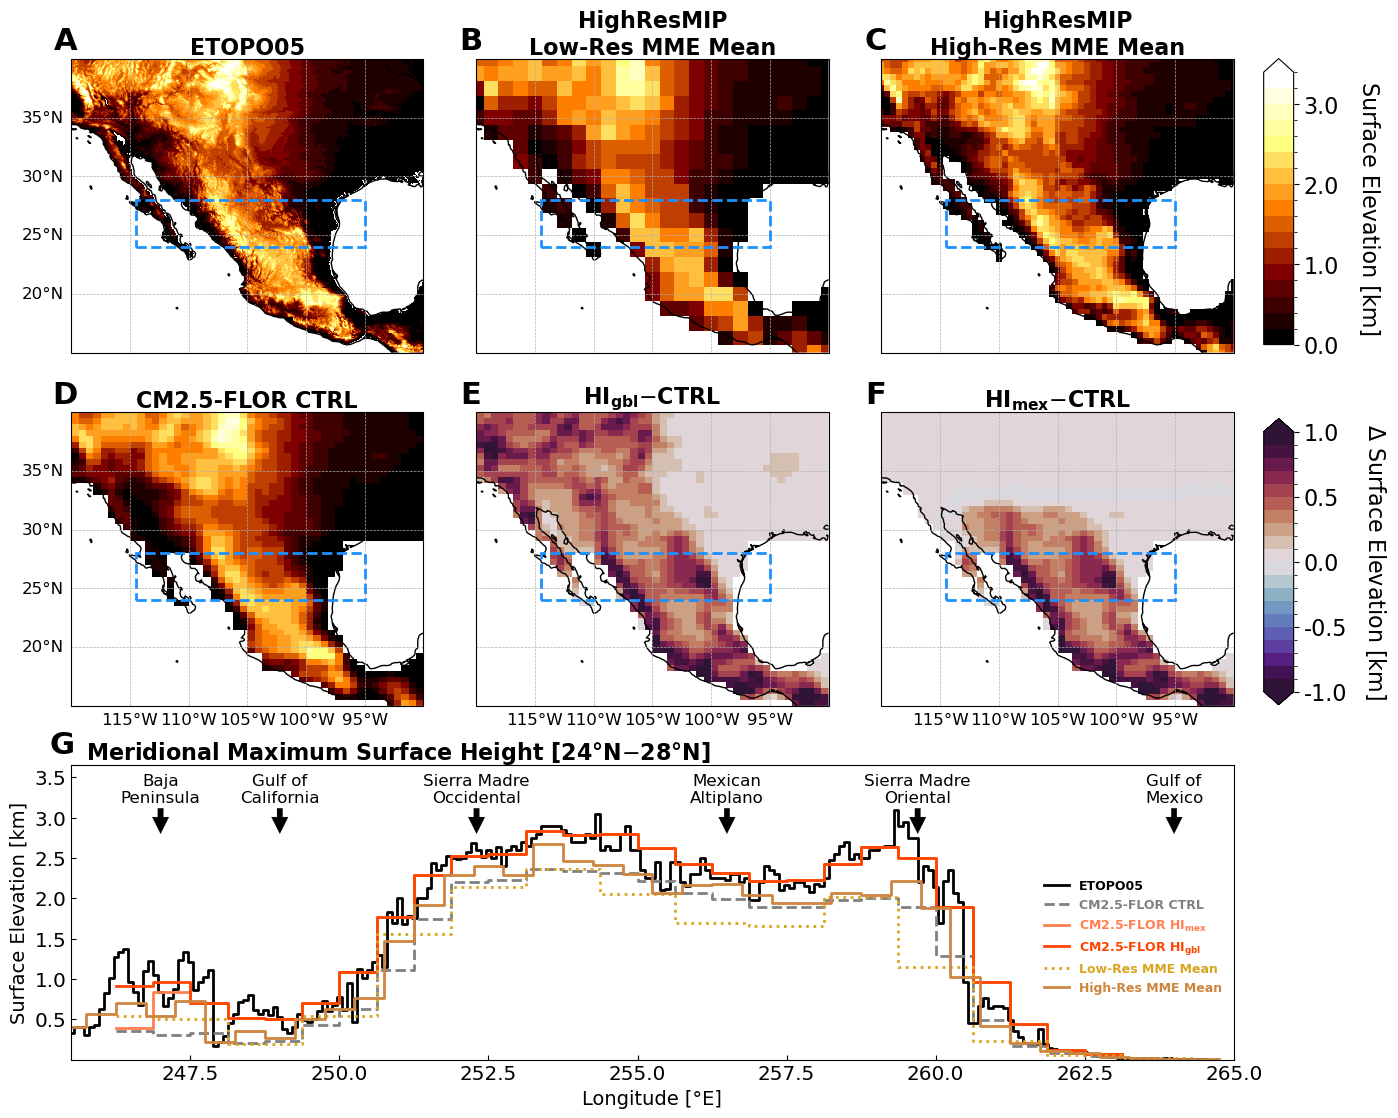
\includegraphics[width=\textwidth]{figs/fig_1_topo_swna_maps_profiles_etopo_hrmip-median_gfdl.png}
    \caption{\textbf{Comparison of observed topography and model boundary conditions in the southwestern U.S. and Mexico.} Spatial distribution of land elevation for (a) ETOPO05 observations at its native 5' resolution, (b) ETOPO05 interpolated to HighResMIP low-resolution ensemble median resolution (125 km), (c) ETOPO05 interpolated to HighResMIP high-resolution ensemble median resolution (50 km), and (d) CM2.5-FLOR CTRL (nominal resolution of 50 km). The change in surface elevation in the CM2.5-FLOR modified topography experiments relative to CTRL is shown for (e) HI$_{gbl}$ and (f) HI$_{mex}$. (g) Zonal profile of meridional maximum topography (between 24\textdegree{N}--29\textdegree) across a transect of the Baja Peninsula-Sierra Madre Occidental delineated by the dashed blue box on panels (a)--(f).}
    \label{fig:topo}
\end{figure}

The CM2.5-FLOR perturbed topography experiments were first presented in \citeA{baldwin21a} and detailed descriptions of the simulations can be found therein. The surface height boundary conditions implemented in the model include: (1) CTRL, the control experiment that uses the standard CM2.5-FLOR surface height boundary condition, (2) HI$_{gbl}$ wherein global topography was elevated to the sub-grid-cell maximum (rather than mean as in the CTRL boundary condition), and (3) HI$_{mex}$ wherein topography only over Central America and Mexico (between 14\textdegree{N}--32\textdegree{N}, 113\textdegree{W}--85\textdegree{W} and 5\textdegree{N}--14\textdegree{N}, 95\textdegree{W}--75.5\textdegree{W}) was elevated to the sub-grid-cell maximum while the rest of the world's topography reflects the standard (i.e., CTRL) boundary condition. Sub-grid-cell topography for HI$_{gbl}$ and HI$_{mex}$ was derived from ETOPO05. This ``maximum'' scheme better aligns the model's topographic peak heights with observations, though it is important to note that, while the re-gridding is volume conservative, observed absolute peak heights are still higher than the model in several places due to the conversion of the rectilinear ETOPO05 data to the cubed sphere model grid. A comparison of topography in ETOPO05 at its native resolution and as represented in the CTRL boundary condition, in addition to the increase in surface height in HI$_{gbl}$ and HI$_{mex}$ relative to CTRL, is depicted in Figure \ref{fig:topo}a,d--f. %The profile highlights the degree to which model topographic boundary conditions capture the complex terrain across the Baja California Peninsular Range, Gulf of California, Sierra Madre Occidental, Mexican Altiplano, and Sierra Madre Oriental.

The initial mass of the atmosphere is unchanged in the elevated topography experiments. As topography displaces air, the global means of simulated atmospheric pressure fields is higher in simulations forced with HI$_{gbl}$ and HI$_{mex}$ topography than CTRL. We thus first subtract the global mean from the field to facilitate comparison of some quantities (i.e., sea level pressure) across simulations.

Each of the 3 surface height boundary conditions were tested under Preindustrial and elevated CO$_2$ conditions. Preindustrial simulations were forced with 1860 CE radiative forcings and run for at least 200 years; we use model years 100-199 to calculate climatologies for consistency across simulations of different lengths. Future changes to the NAM in CM2.5-FLOR due to greenhouse gas forcing were simulated under 2$\times$CO$_2$ conditions. In these experiments, beginning in simulation year 101, atmospheric CO$_2$ concentrations were increased at 1\% per year until reaching doubling, then run for an additional several hundred years with the radiative forcing held constant at 2$\times$CO$_2$; we calculate climatologies from years 200-299. 

%% -------------------
\subsection{NAM sub-domains}
%% -------------------
The center of NAM activity is located over northwest Mexico and the system typically only reaches as far north as southern Arizona and southwestern New Mexico. At times, however, the system can intensify and additionally influence a broader swath of the western U.S., extending westward into California and northwards across Utah and Colorado. Although the climatology of the core system (spanning northwest Mexico and southern Arizona/New Mexico) is often discussed holistically, the spatiotemporal patterns of seasonal precipitation in northwestern Mexico versus the southwestern U.S. are actually also distinct in nature. Accordingly, we separate our analyses and discussion to view these two sub-domains of the core NAM region in isolation. We define the ``Southern Domain'' as an obliquely oriented region spanning approximately 20–30\textdegree{N} and 112–102\textdegree{W}, encompassing the mountainous terrain of northwest Mexico and adjacent lowlands and Gulf of California (Figure S1, light red box). We then define the ``Northern Domain'' as the region spanning 29.5–35.5\textdegree{N} and 114.5–106.5\textdegree{W}, encompassing the lower-elevation terrain north of the Sierra Madre Occidental near the Mexico–U.S. border and across southern Arizona and New Mexico (Figure S1, dark red box)

% ======================================================== %
% RESULTS
% ======================================================== %
\section{Results}
%% -------------------
\subsection{Role of horizontal resolution on NAM precipitation biases}
%% -------------------
The low- and high-resolution configurations of HighResMIP models differ in their ability to simulate the spatial distribution of Jul.--Sept. precipitation (Figures \ref{fig:hrmip-biases}, S2) as well as the magnitude of the seasonal peak in climatological monthly precipitation averaged over the NAM sub-domains (Figure S4). These differences in NAM biases between the resolution ensemble means are robust when evaluated against various precipitation products.

In the Southern Domain, models with zonal grid-spacing $\sim$1\textdegree{} or coarser simulate, on average, too-little precipitation overall, though a few select models overestimate precipitation over the Gulf of California (Figure \ref{fig:hrmip-biases}d blue lines, e). Though high-resolution models similarly underestimate rainfall over low-lying areas, the negative bias is more pronounced and confined closer to the eastern shore of the Gulf of California in the high-resolution compared to the low-resolution ensemble mean. Unlike the low-resolution configurations, however, the majority of high-resolution configurations overestimate rainfall rates along the windward slopes of the Sierra Madre Occidentals at elevations $>$800 m (Figure \ref{fig:hrmip-biases}d red lines, f). Yet, as the magnitude of the models' dry biases over the low-lying areas west of the Sierra Madre Occidental is typically greater than their wet biases over the higher elevation terrain, the domain-mean bias is still negative for most models (Figure \ref{fig:hrmip-biases}d, high-res. MME profile). As such, though the majority of the low- and high-resolution HighResMIP models exhibit a mean dry bias in the Southern Domain, there is, in actuality, a markedly different spatial structure in the rainfall bias in the high-resolution configurations compared to their low-resolution counterparts. This difference is chiefly that the dry bias is more-or-less uniform in the low-resolution configurations but there is a dipole of dry and wet biases in the high-resolution configurations.

\begin{figure}[!htbp]
    \centering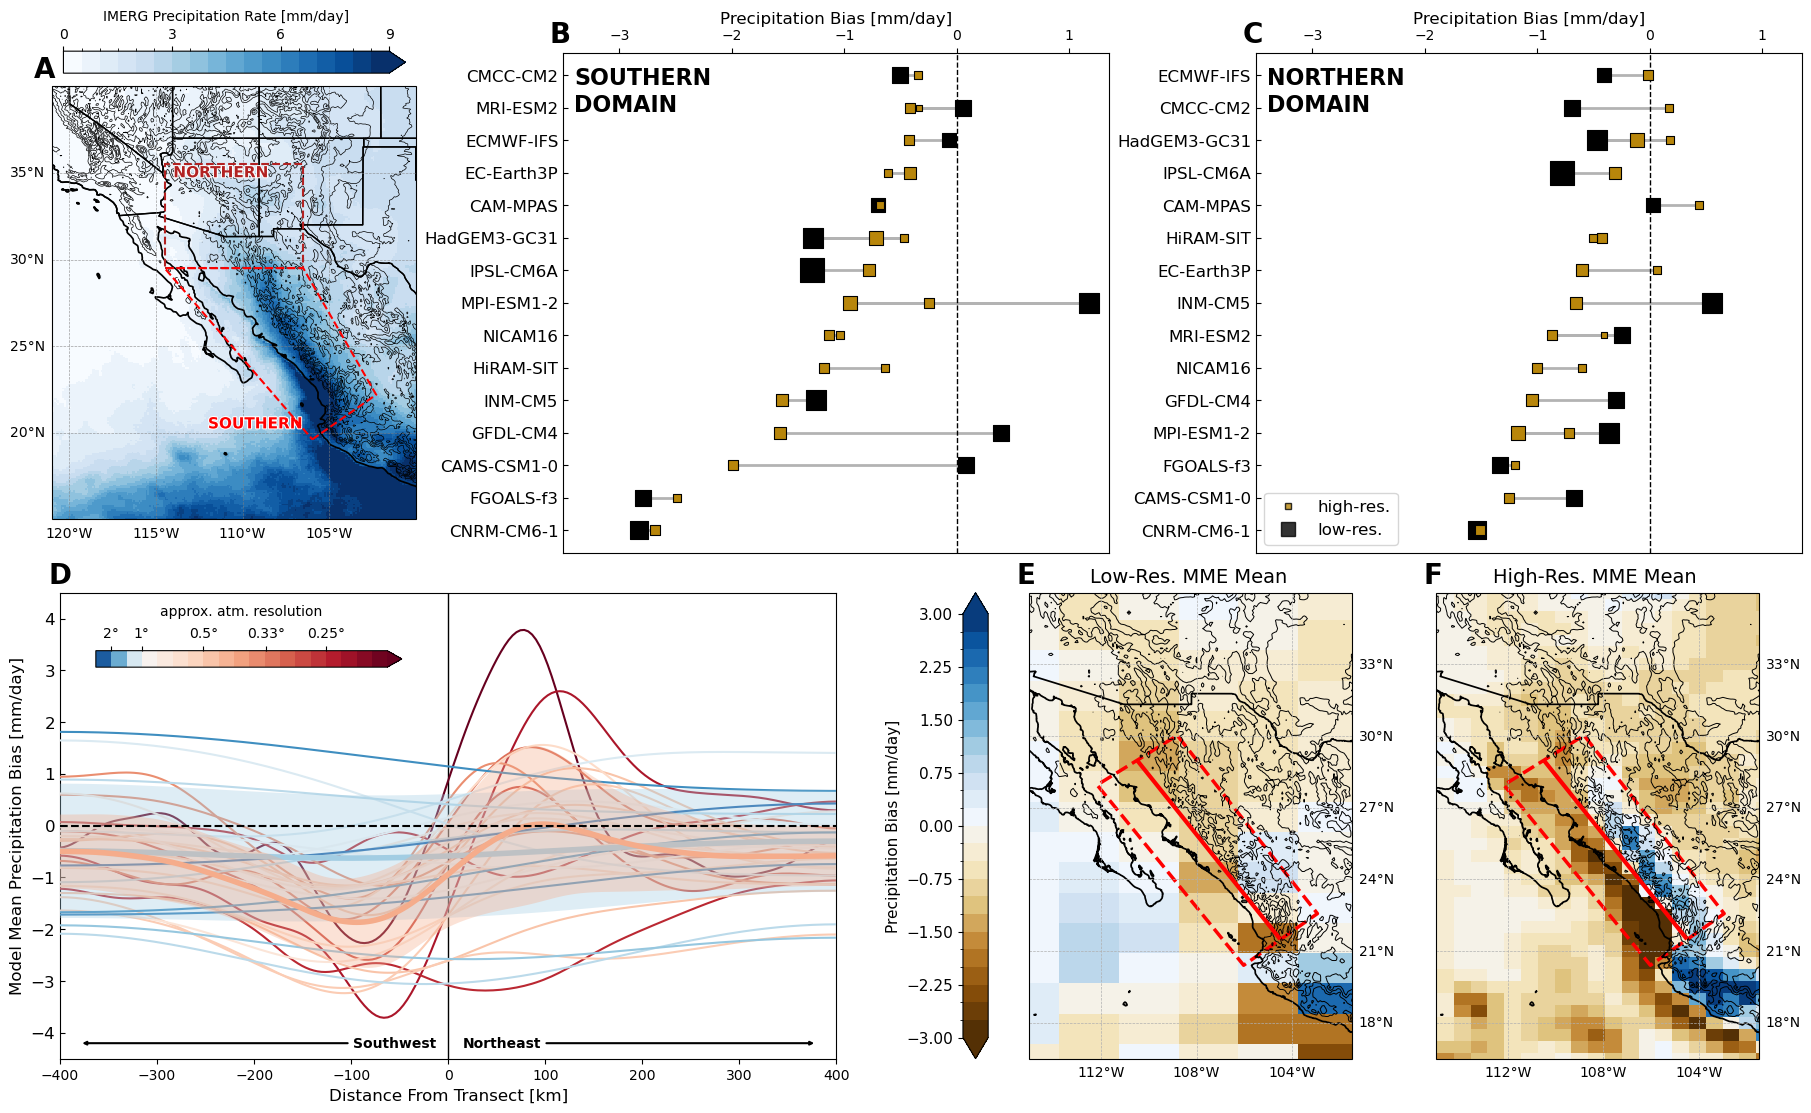
\includegraphics[width=\textwidth]{figs/fig_2_prec_hrmip_historical_change_profiles_imerg.png}
    \caption{\textbf{Character of NAM precipitation biases in HighResMIP models.} (a) Observed spatial distribution of climatological  precipitation from IMERG \cite<2001--2018;>{huffman20} with dashed boxes outlining the Northern (dark red) and Southern (light red) Domains. HighResMIP models' domain-mean precipitation biases (calculated as the model minus IMERG) for the (b) Southern and (c) Northern Domains. (d) Profiles of HighResMIP models' precipitation biases in northwest Mexico, 400 km southwest and northeast (dashed red box on panels e--f) of a transect line oriented parallel to the windward slopes of the Sierra Madre Occidental (at $\sim$800 m, from 29\textdegree{N}, 249.75\textdegree{E} to 22\textdegree{N}, 254.75\textdegree{E}; thick red line on panels e--f is the transect line and dashed red box indicates the limits of the 400 km normal distance). Individual model bias profiles are plotted as thin colored lines while the multi-model ensemble (MME) mean bias profiles are plotted as thicker lines with shading for the 1$\sigma$ standard deviation capturing the spread across resolution ensemble members. Line colors correspond to the models' approximate grid-spacing inferred from their longitude dimension length. Profiles created by first calculating binned precipitation biases along a common distance axis then applying a Gaussian smoothing filter with a scale set by each model's native grid-spacing. Spatial patterns of the MME mean precipitation biases for the (e) low-resolution ($\geq\sim$1\textdegree{}) and (f) high-resolution ($<$1\textdegree{}) ensembles. Thin black contours on panels a, e, and f are ETOPO05 topography between 800 m to 3800 m, intervals of 500 m. All panels are based on Jul.--Sept. mean precipitation.}
    \label{fig:hrmip-biases}
\end{figure}

Our finding that low-resolution configurations exhibit drier-than-observed precipitation across the majority of the Southern Domain is consistent with prior work suggesting the representation of topography on model grids coarser than $\sim$100 km is insufficient to capture the terrain-forced low-level circulation of the NAM \cite{berbery03jc,pascale16jc,varuolo-clarke19jc}. The Sierra Madre Occidental act as a lifting mechanism that converts enthalpy ($E$) to moist static energy ($h$) \cite{varuolo-clarke19jc,boos21n}. Too-low topography in this region may thus lead to weak or absent orographically-forced convection in coarse-resolution models. As standard practice for generating model topographic boundary conditions is to use grid-cell-averages of observed topography, finer-resolution model grids have more irregular topography with higher peak heights (e.g., Figure \ref{fig:topo}g,h). Indeed, coarsening observed topography in northwest Mexico from the product's native 5-minute resolution to 100 km or 200 km lowers Sierra Madre Occidental peak heights by an average of $\sim$400 m or $\sim$570 m, respectively, compared to $\sim$280 m when mapped to a 50 km resolution grid (Figure S5, Supplementary Text S1). Improvement in the representation of Sierra Madre Occidental peak heights at finer model resolutions should therefore result in more realistic simulation of orographic precipitation characteristic of the NAM in its Southern Domain. 

Consistent with this expectation, we find that the HighResMIP high-resolution ensemble members have greater precipitation rates over the Sierra Madre Occidental compared to the low-resolution members (Figure S2). Nevertheless, there is overall mixed domain-mean improvement in the simulation of precipitation with resolution (8 of 15 model families show reduced biases, Figure \ref{fig:hrmip-biases}b) and the precipitation maxima associated with the impact of the Sierra Madre Occidental on orographically-forced convection are located too far upslope and inland \ref{fig:hrmip-biases}d,f). For models with multiple high-resolution configurations, the more moderate refinement in resolution actually worsens the model's dry bias over the Gulf of California moreso than enhances orographic precipitation; the strongest rainfall rates along the Sierra Madre Occidental slopes generally occur in the highest-resolution configurations (Figures \ref{fig:hrmip-biases}d, S1). As such, the highest-resolution models thus often appear to have domain-averaged rainfall rates that are closer to observations than the low-resolution models (Figure \ref{fig:hrmip-biases}b). However, this is a consequence of the overestimated rainfall rates over the Sierra Madre Occidental that effectively negate the impact of underestimated rainfall rates over the Gulf of California on the magnitude of the domain-mean bias. 

Interestingly, though the high-resolution ensemble members simulate a broadly more realistic spatial structure of the NAM in the Southern Domain compared to the low-resolution ensemble members, the multi-model ensemble mean of biases from both configuration ensembles exhibit similar dry bias magnitudes ($\sim$-0.5 to -2 mm/day) in the Northern Domain (Figure \ref{fig:hrmip-biases}b,c). This suggests that better simulating rainfall rates along the Sierra Madre Occidental does not necessarily correspond to improved simulation of NAM rainfall in the Northern Domain. In comparing the impact of increasing spatial resolution within single model families, \citeA{varuolo-clarke19jc} and \citeA{pascale16jc} found that the higher-resolution configurations of the CAM5 and GFDL-CM2 models, respectively, had more realistic northward penetration of NAM moisture into the southwest U.S. than their lower-resolution configurations. We find, however, that this impact of enhanced model spatial resolution does not hold across a broader model ensemble; of the 15 model families that contributed to HighResMIP, 7 model families actually show no change or a worsening of Northern Domain precipitation biases following resolution refinement (Figure \ref{fig:hrmip-biases}c).


%% -------------------
\subsection{Influence of elevated topography on NAM simulation at high-resolutions in CM2.5-FLOR}
%% -------------------
We turn to the CM2.5-FLOR simulations to better understand the role of topography in shaping the remaining NAM precipitation biases in the HighResMIP high-resolution ensemble. These experiments provide insight to whether or not topographic peak heights in the high-resolution configurations are yet sufficient for capturing realistic orographic blocking patterns; prior work has shown orographic blocking by narrow mountain ranges can be underestimated even in GCMs with 50 km resolution \cite{baldwin21a}. The 50 km nominal resolution of CM2.5-FLOR is identical to the median resolution of the HighResMIP high-resolution ensemble such that the we can interpret the CTRL simulation as having comparable limitations in its resolution of topographic peak heights and orographic blocking, as exemplified in the topographic profiles in Figure \ref{fig:topo}g. We interpret the overall sensitivity of NAM simulation to topographic forcing with the HI$_{gbl}$ experiment. HI$_{mex}$, in which topography was only elevated to the sub-grid-cell maximum over Mexico and Central America, provides a lens for diagnosing which elements of topography specifically drive the shifts in HI$_{gbl}$. Below, we first describe how elevating different elements of topography influences NAM rainfall in CM2.5-FLOR, then explore their impacts on local and large-scale circulation drivers of the NAM. % add line about robustness of results, shown in Figure S4 for the CM2.5-FLOR experiments.

%% -------------------
\subsubsection{Changes in simulated precipitation biases}
The Preindustrial CM2.5-FLOR experiment forced with CTRL topography also exhibits a dipole of precipitation biases in the Southern Domain---with too-little precipitation over the Gulf of California and the lower Sierra Madre Occidental slopes in contrast to too-much precipitation over the Sierra Madre Occidental peaks---consistent with the bias pervasive among the high-resolution configurations of HighResMIP models (c.f., Figures \ref{fig:flor-prec}a, S6 and Figures \ref{fig:hrmip-biases}f, S2). In HI$_{gbl}$, there is an increase of precipitation over most of the windward Sierra Madre Occidental slopes below $\sim$3 km elevation (Figure \ref{fig:flor-prec}b). This corresponds to a reduction of CM2.5-FLOR's dry bias along the lower ($<$1 km masl) slopes, but an exacerbation of the wet bias at the higher elevations (Figure \ref{fig:flor-prec}b, hatching). Drying in the range's higher elevations does occur in HI$_{gbl}$ south of $\sim$25\textdegree{N}, reducing wet biases there. In the Northern Domain, elevated topography in HI$_{gbl}$ also led to higher rainfall rates across most of Arizona and New Mexico (Figure \ref{fig:flor-prec}b). This represents a reduction of the model's dry bias in Arizona south of the Mogollon Rim (which is the southwestern edge of the Colorado Plateau), although similarly exacerbates existing wet biases over the higher elevations of the North American Cordillera (Figure \ref{fig:flor-prec}b, hatching).

\begin{figure}[!htbp]
    \centering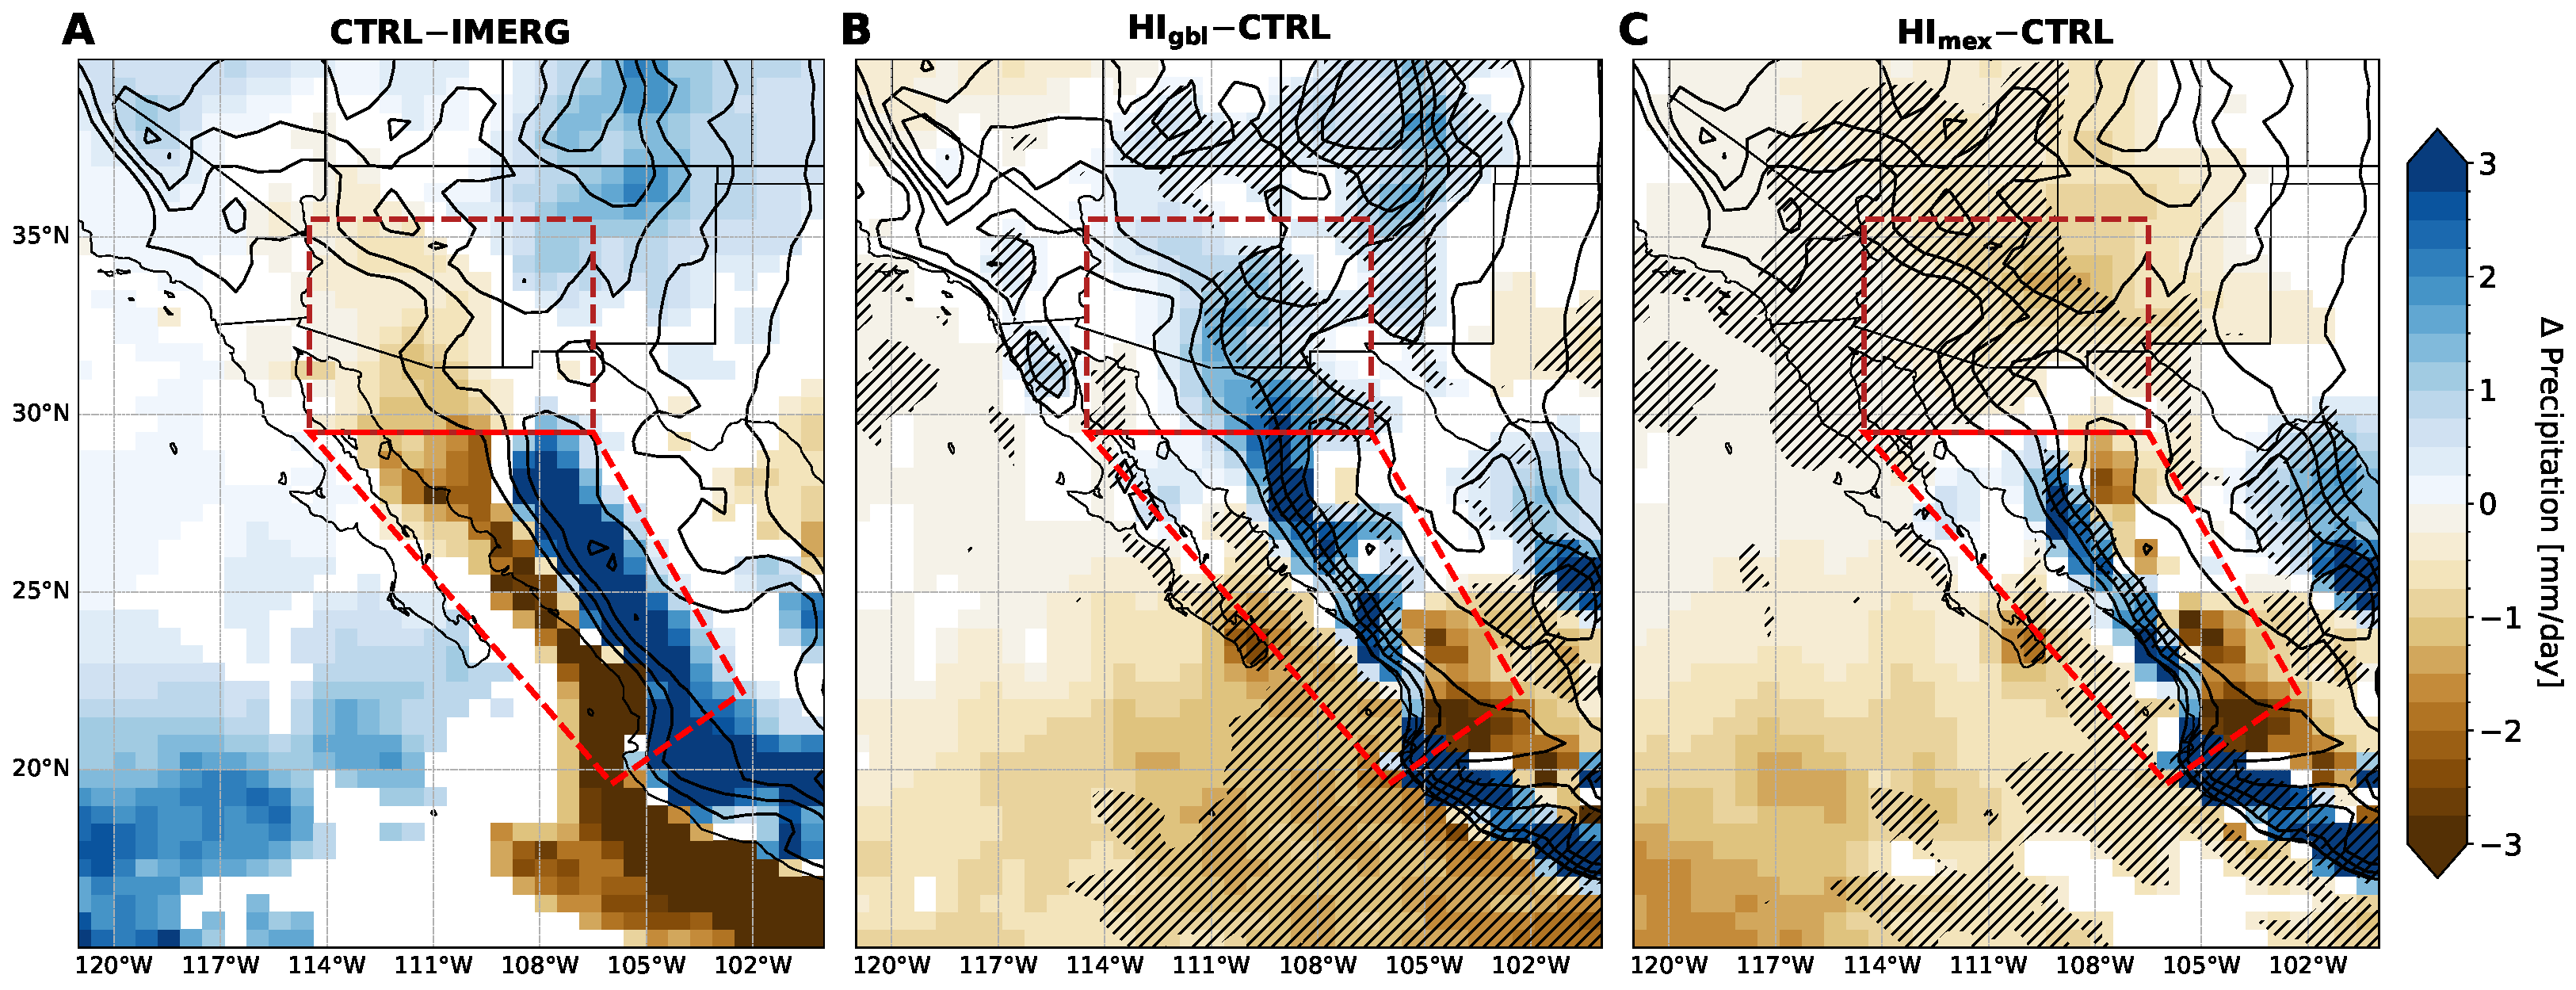
\includegraphics[width=\textwidth]{figs/fig_3_prec_flor_pi_imerg-bias_change.pdf}
    \caption{\textbf{Impact of elevated topography on simulated NAM precipitation in CM2.5-FLOR.} Differences between simulated Jul.--Sept. precipitation (shading) for (a) CM2.5-FLOR CTRL minus IMERG observations, (b) HI$_{gbl}$ minus CTRL, and (c) HI$_{mex}$ minus CTRL. Fields are masked where the difference is statistically insignificant (p$>$0.1) based on a two-sided Welch's t-test in panel a and two-sided student's t-test in panels b--c. Hatching indicates where a statistically significant change in precipitation in HI$_{gbl}$ or HI$_{mex}$ results in simulated rainfall rates with a higher magnitude bias (vs. IMERG) than in the CTRL simulation. Thin black contours outline model topography from 800 m to 3800 m, intervals of 500 m. Dashed boxes outline the Northern (dark red) and Southern (light red) Domains.}
    \label{fig:flor-prec}
\end{figure}

Implementing grid-cell maximum topography only in Mexico/Central America in HI$_{mex}$ raises precipitation along the lower Sierra Madre Occidental's slopes and reduces it along the range peaks (Figure \ref{fig:flor-prec}c). HI$_{mex}$ thus better reduces the contrasting precipitation biases in northwest Mexico compared to HI$_{gbl}$. Despite the improved representation of precipitation in the Southern Domain in HI$_{mex}$, there is little improvement in CM2.5-FLOR's dry bias in the Northern Domain. HI$_{mex}$ actually exhibits a larger pattern of drying across the western U.S. that extends from the Pacific coast to the Rocky Mountains. Though this drying counteracts the CTRL wet bias over the Rocky Mountains and Colorado Plateau regions across Colorado and New Mexico, it is an exacerbation of the existing dry NAM rainfall biases in the Northern Domain Colorado Plateau region of Arizona and the low-lying desert regions of southeastern California and Arizona. 

%% -------------------
\subsubsection{Impacts on NAM circulation features that drive Southern Domain precipitation}

\begin{figure}[!htbp]
    \centering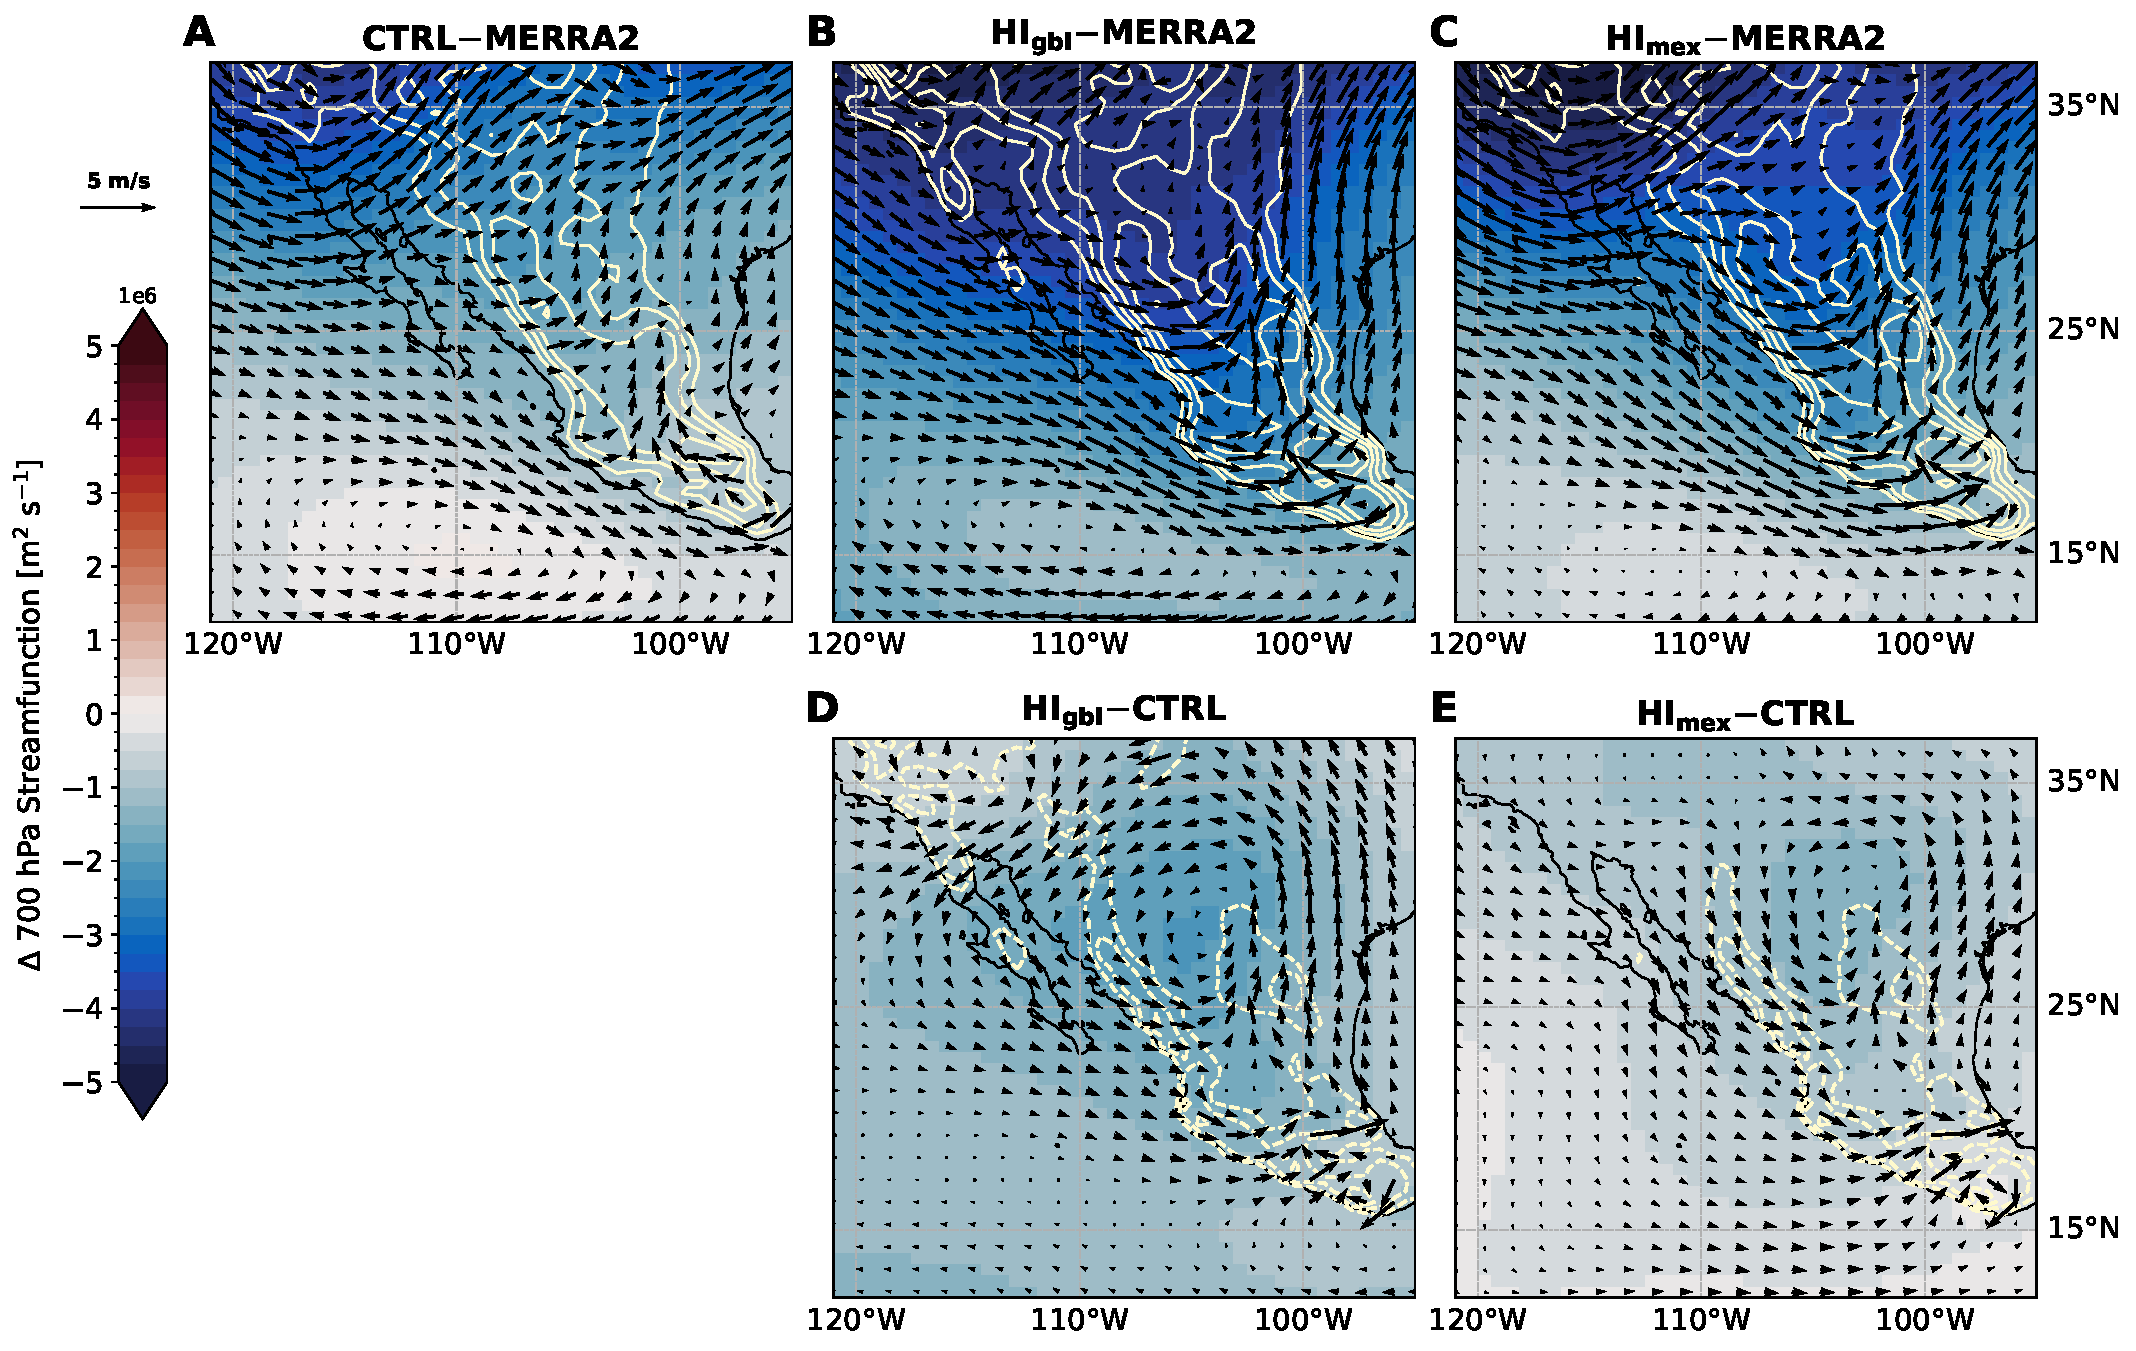
\includegraphics[width=1\textwidth]{figs/fig_4_psi-700hpa_merra2-bias_change_flor_pi.pdf}
    \caption{\textbf{Impact of elevated topography on lower-troposphere circulation and streamfunction in CM2.5-FLOR.} Jul.--Sept. seasonal mean biases relative to MERRA-2 reanalysis for 700 hPa streamfunction ($\Psi_{700}$, shading) and wind velocity (vectors) calculated from $U$ and $V$ wind components in the Preindustrial CM2.5-FLOR (a) CTRL, (b) HI$_{gbl}$, and (c) HI$_{mex}$ simulations. Change in $\Psi_{700}$ and wind velocities in CM2.5-FLOR due to elevating topography relative to CTRL for (d) HI$_{gbl}$, and (e) HI$_{mex}$. Solid light yellow contours on a--c are topography from 800 m to 3800 m at intervals of 500 m; dashed light yellow contours on d--e are the change in topography from 500 m to 1500 m at intervals of 250 m. Fields are not masked for statistical significance.}
    \label{fig:flor-700hpa-psi}
\end{figure}

Though the location of the climatological precipitation maxima spanning the lower-middle slopes of the Sierra Madre Occidental is somewhat improved in CM2.5-FLOR after implementing elevated topography, precipitation becomes more positively biased over their upper slopes. One hypothesis for this persistent misalignment relative to observations is misrepresentation of the large-scale circulation that interacts with these mountains \cite{berbery01jc,boos21n}. To evaluate this, we compare model biases of the 700 hPa wind field and its streamfunction in CTRL, HI$_{gbl}$, and HI$_{mex}$ in Figure \ref{fig:flor-700hpa-psi}a--c. CTRL exhibits a low pressure bias that manifests as a trough over southwestern North America; this trough deepens and extends further to the southeast over Mexico in response to higher surface elevation (Figure \ref{fig:flor-700hpa-psi}b,c vs. a). Consequently, the winds impinging on the Sierra Madre Occidental in the elevated topography simulations are overly strong and westerly. \citeA{boos21n} conducted idealized experiments with and without the existence of the Sierra Madre Occidental and found that the range mechanically forces a stationary wave pattern at 700 hPa that drives westerly, upslope flow. The changes in circulation depicted in Figure \ref{fig:flor-700hpa-psi}d,e are consistent with the mechanism described in \citeA{boos21n}, but are a clear exacerbation of existing biases, possibly due to the combined effects of exaggerated orography and surface heating in HI$_{gbl}$ and HI$_{mex}$ on the summertime stationary wave \cite{ringler99jas}. The anomalous westerly flow windward of the Sierra Madre Occidental in HI$_{gbl}$ and HI$_{mex}$ likely partially compensated for the direct orographic blocking effects of the elevated topographic boundary condition and contributes to the persistence of positive rainfall biases $>\sim$1500 m in CM2.5-FLOR. As the anomalous cyclonic circulation induced by the elevated terrain is stronger and located further to the west over the Mexican Altiplano in HI$_{gbl}$ than in HI$_{mex}$, this mechanism may additionally explain the greater reduction of precipitation along the Sierra Madre Occidental peaks in HI$_{mex}$ compared to HI$_{gbl}$. 


%% -------------------
\subsubsection{Impacts on NAM circulation features that drive Northern Domain moistening}
To understand the improved simulation of precipitation in the Northern Domain in HI$_{gbl}$, we examine changes in the GoCLLJ, which plays a key role driving rainfall in this region. The CTRL simulation of CM2.5-FLOR exhibits too-weak southerly flow over the northern Gulf of California (Figure \ref{fig:flor-slp-llj}a), which suggests reduced moisture inflow and is consistent with the dry bias in the Northern Domain (Figure \ref{fig:flor-prec}a). The too-weak GoCLLJ appears to be a consequence of too high SLP over the low deserts of the southwest U.S. (Figure \ref{fig:flor-slp-llj}a). In HI$_{gbl}$, there is an overall reduction in SLP, though the lowering of SLP is deepest near the Arizona-Mexico border just north of the Gulf of California (Figure \ref{fig:flor-slp-llj}b). This relative lowering of SLP north of the Gulf compared to at its opening in the south corresponds to an increase in the along-Gulf SLP gradient (Figure \ref{fig:flor-slp-llj}d). The enhanced SLP gradient is additionally accompanied by an intensification of the southerly low-level winds flowing from the northern Gulf of California into the southwestern U.S. at 925 hPa (Figure \ref{fig:flor-slp-llj}b). Though elevating the Sierra Madre Occidentals in HI$_{mex}$ results in a modest reduction in SLP over the southwest U.S., SLP at the southern end of the Gulf is similarly reduced. Consistent with a small net change in along-Gulf SLP gradient, there is a lack of any significant increase in the seasonal mean southerly wind strength associated with the GoCLLJ over the northern Gulf (Figure \ref{fig:flor-slp-llj}c).

\begin{figure}[!htbp]
    \centering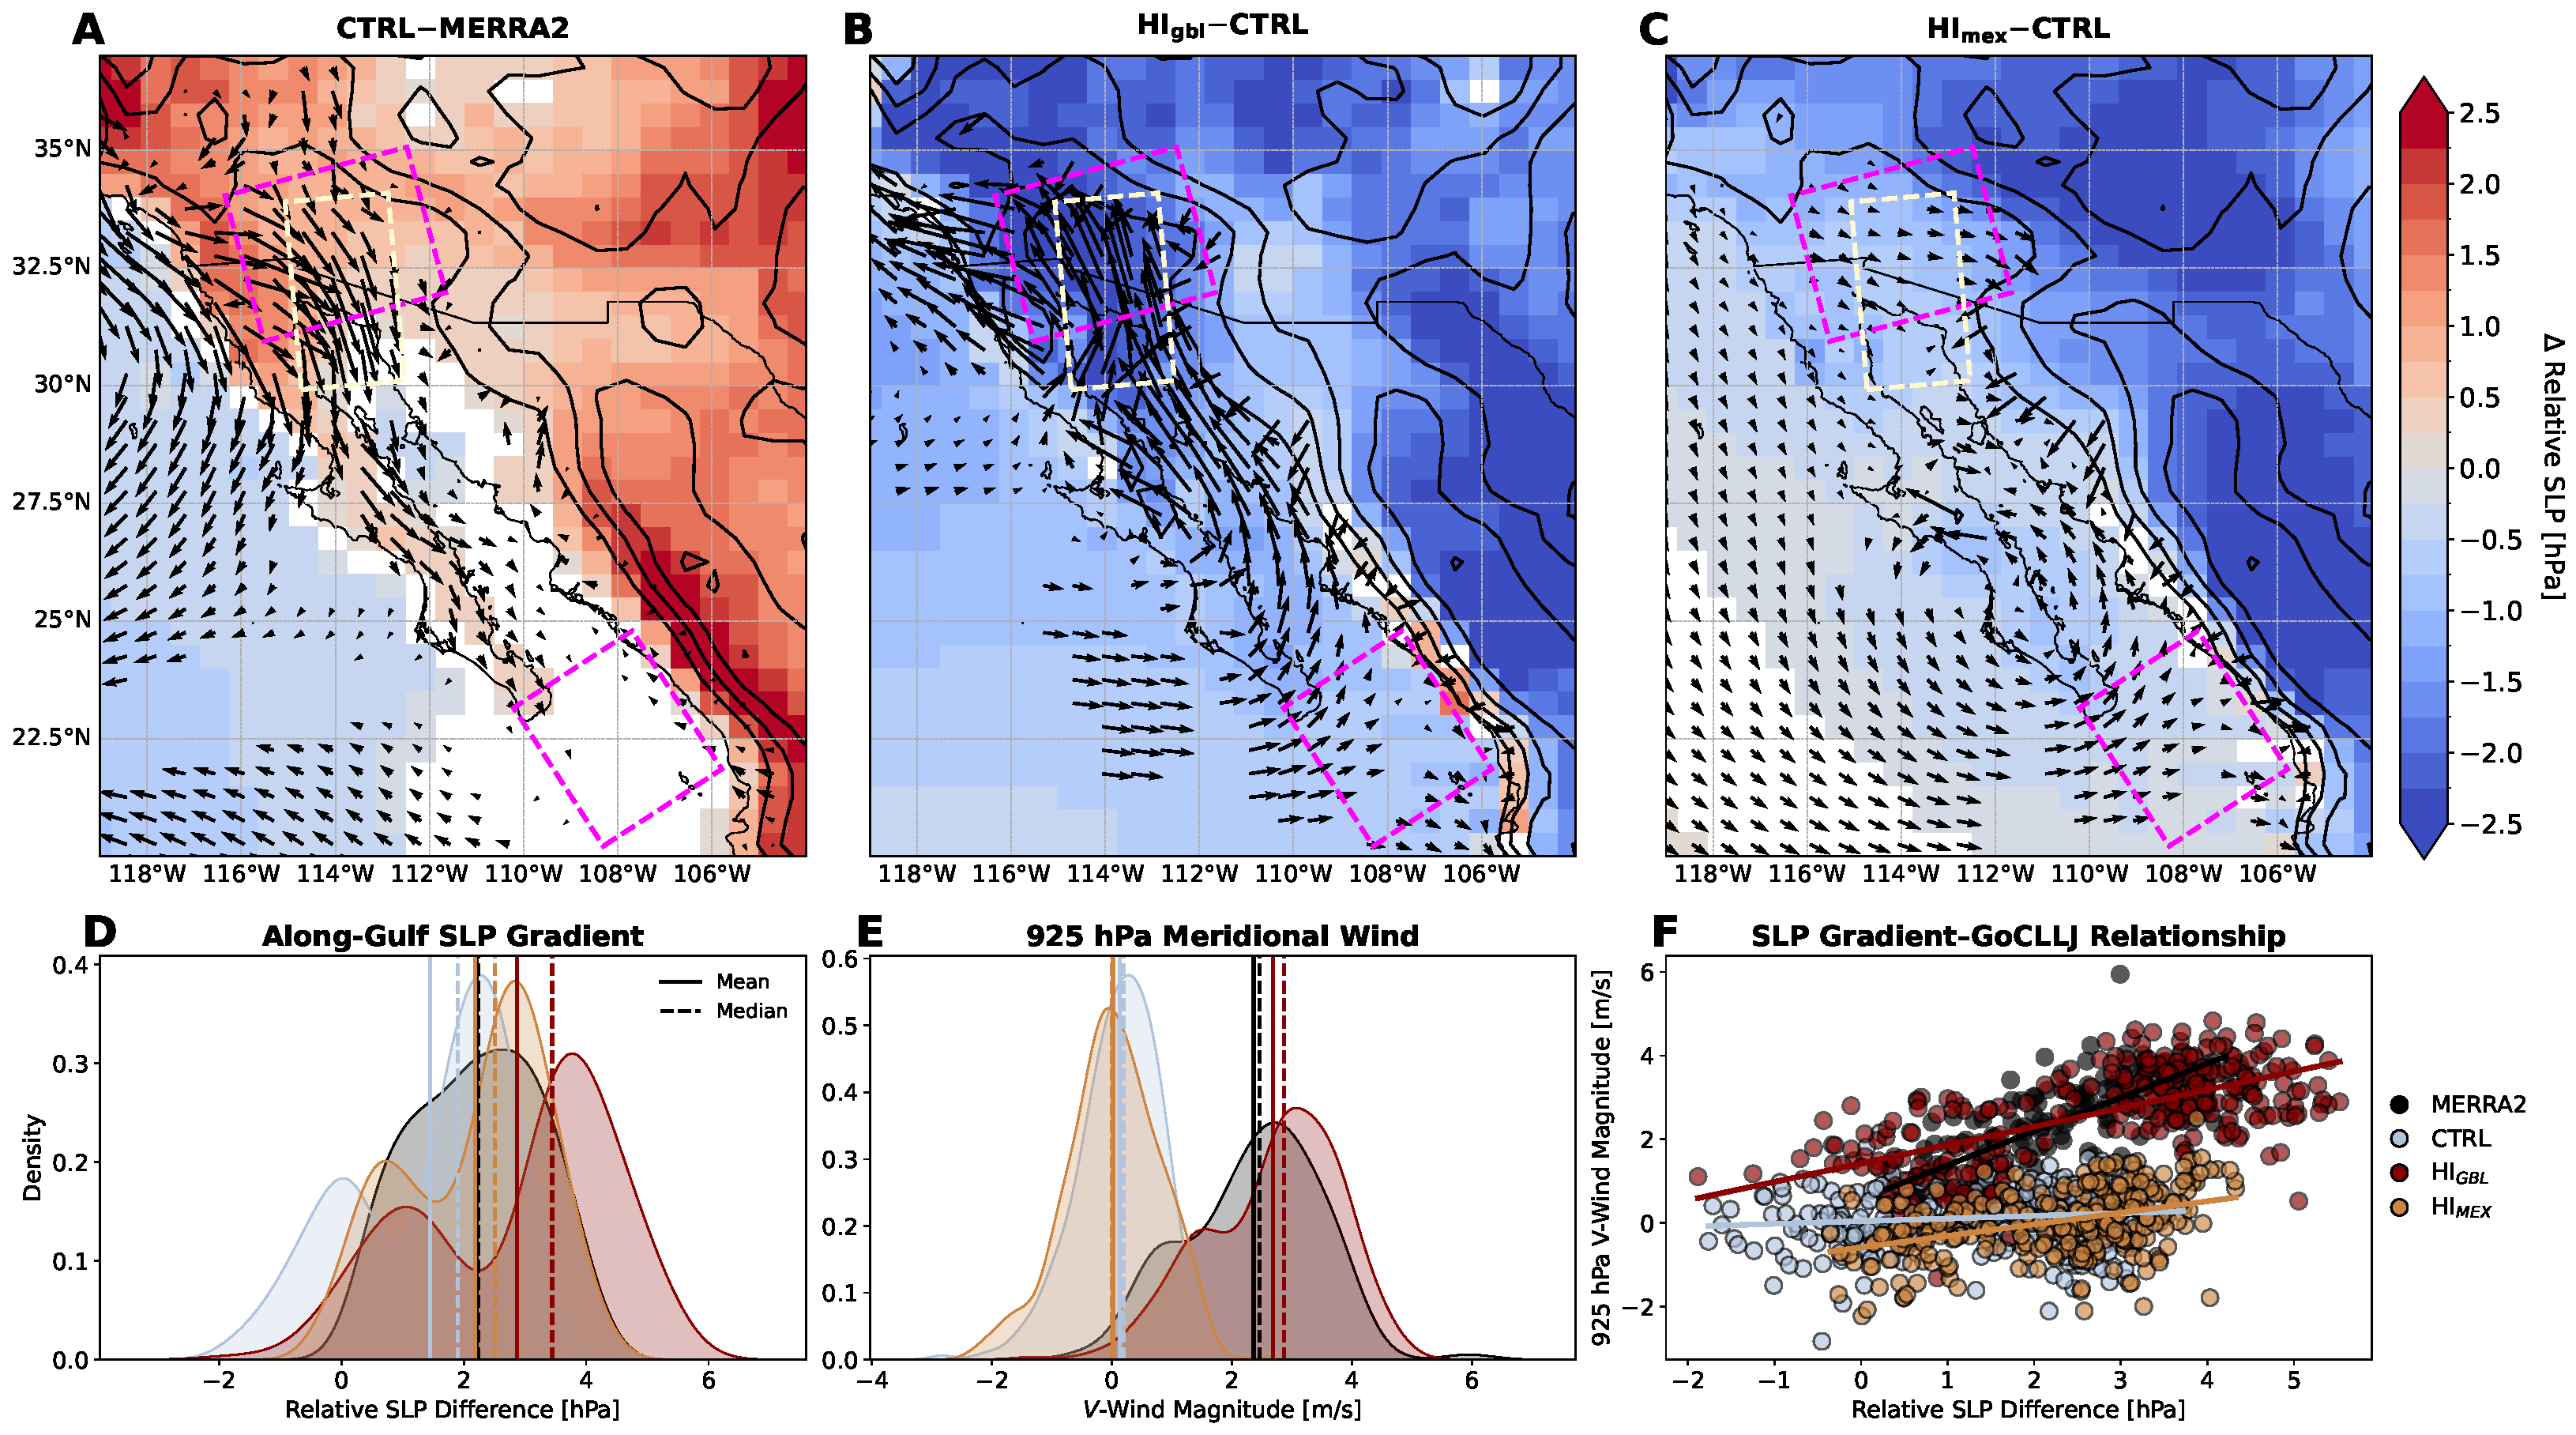
\includegraphics[width=1\textwidth]{figs/fig_5_slpa_925wind_merra2-bias_change_flor_pi.pdf}
    \caption{\textbf{Impact of elevated topography on sea level pressure gradients and near-surface circulation in CM2.5-FLOR.} Differences between simulated Jul.--Sept. sea level pressure (SLP) anomalies relative to the global mean (shading) and 925 hPa wind velocity (vectors) for (a) CM2.5-FLOR CTRL minus MERRA-2 reanalysis, (b) HI$_{gbl}$ minus CTRL, and (c) HI$_{mex}$ minus CTRL. Fields are masked where the difference is statistically insignificant (p$>$0.1) based on a two-sided Welch's t-test in panel a and two-sided student's t-test in panels b--c. Distributions of individual July, August, and September monthly mean values across years for (d) along-Gulf SLP gradient (calculated as the north minus south difference of the spatial-mean values within the two dashed magenta boxes on a--c) and (e) 925 hPa meridional wind strength (spatial-mean value within the dashed gold box on a--c), and (f) the relationship between these metrics. Distributions span 1980--2022 for MERRA-2 reanalysis and years 101-200 of the three CM2.5-FLOR Preindustrial experiments.}
    \label{fig:flor-slp-llj}
\end{figure}

In addition to improvements in the seasonal mean state, we also find a more realistic representation of the monthly variability in the along-gulf SLP gradient and the GoCLLJ in the elevated topography simulations, especially HI$_{gbl}$ (Figure \ref{fig:flor-slp-llj}f). While the CTRL SLP gradient distribution is biased too weak, the magnitude of the SLP gradient in HI$_{mex}$ is somewhat increased, and that in HI$_{gbl}$ is further increased and even exaggerated compared to MERRA-2 (Figure \ref{fig:flor-slp-llj}d). Related to the smaller increase in along-Gulf SLP gradient in HI$_{mex}$, there is a slight increase in the maximum 925 hPa winds simulated. However, HI$_{mex}$ still has a marked low bias in wind strength compared to MERRA-2 reanalysis and is not a substantial improvement upon the 925 hPa wind biases in CTRL (Figure \ref{fig:flor-slp-llj}e,f). The distribution of GoCLLJ wind strength in HI$_{gbl}$ is instead remarkably well-aligned with that of the reanalysis. The fact that HI$_{mex}$ exhibits the closest alignment in SLP gradient distributions to MERRA-2, but little improvement in the GoCLLJ distribution relative to that seen in HI$_{gbl}$ (Figure \ref{fig:flor-slp-llj}d,e), suggests these SLP gradients can only partially explain the GoCLLJ changes and one may not be able to directly ascertain how well a model will resolve the GoCLLJ solely by the strength of the along-Gulf SLP gradient \cite{stensrud97mwr,pascale16mwr}. Nonetheless, the HI$_{gbl}$ configuration of CM2.5-FLOR much better captures the relationship between the SLP gradient and low-level meridional wind speeds associated with the GoCLLJ circulation (Figure \ref{fig:flor-slp-llj}f). These changes in the CM2.5-FLOR model are self-consistent in that an increase in low-level wind strength follows increased SLP gradients, yet the absolute magnitude of the SLP gradient needed to produce the magnitude of observed wind speeds is overestimated. Alternatively, the structure of the distribution of 925 hPa meridional winds in Figure \ref{fig:flor-slp-llj}e and their relationship with the along-Gulf SLP gradient in Figure \ref{fig:flor-slp-llj}f suggests that the GoCLLJ is more sensitive to variability in the SLP gradient in HI$_{gbl}$ than HI$_{mex}$.

\begin{figure}[!htbp]
    \centering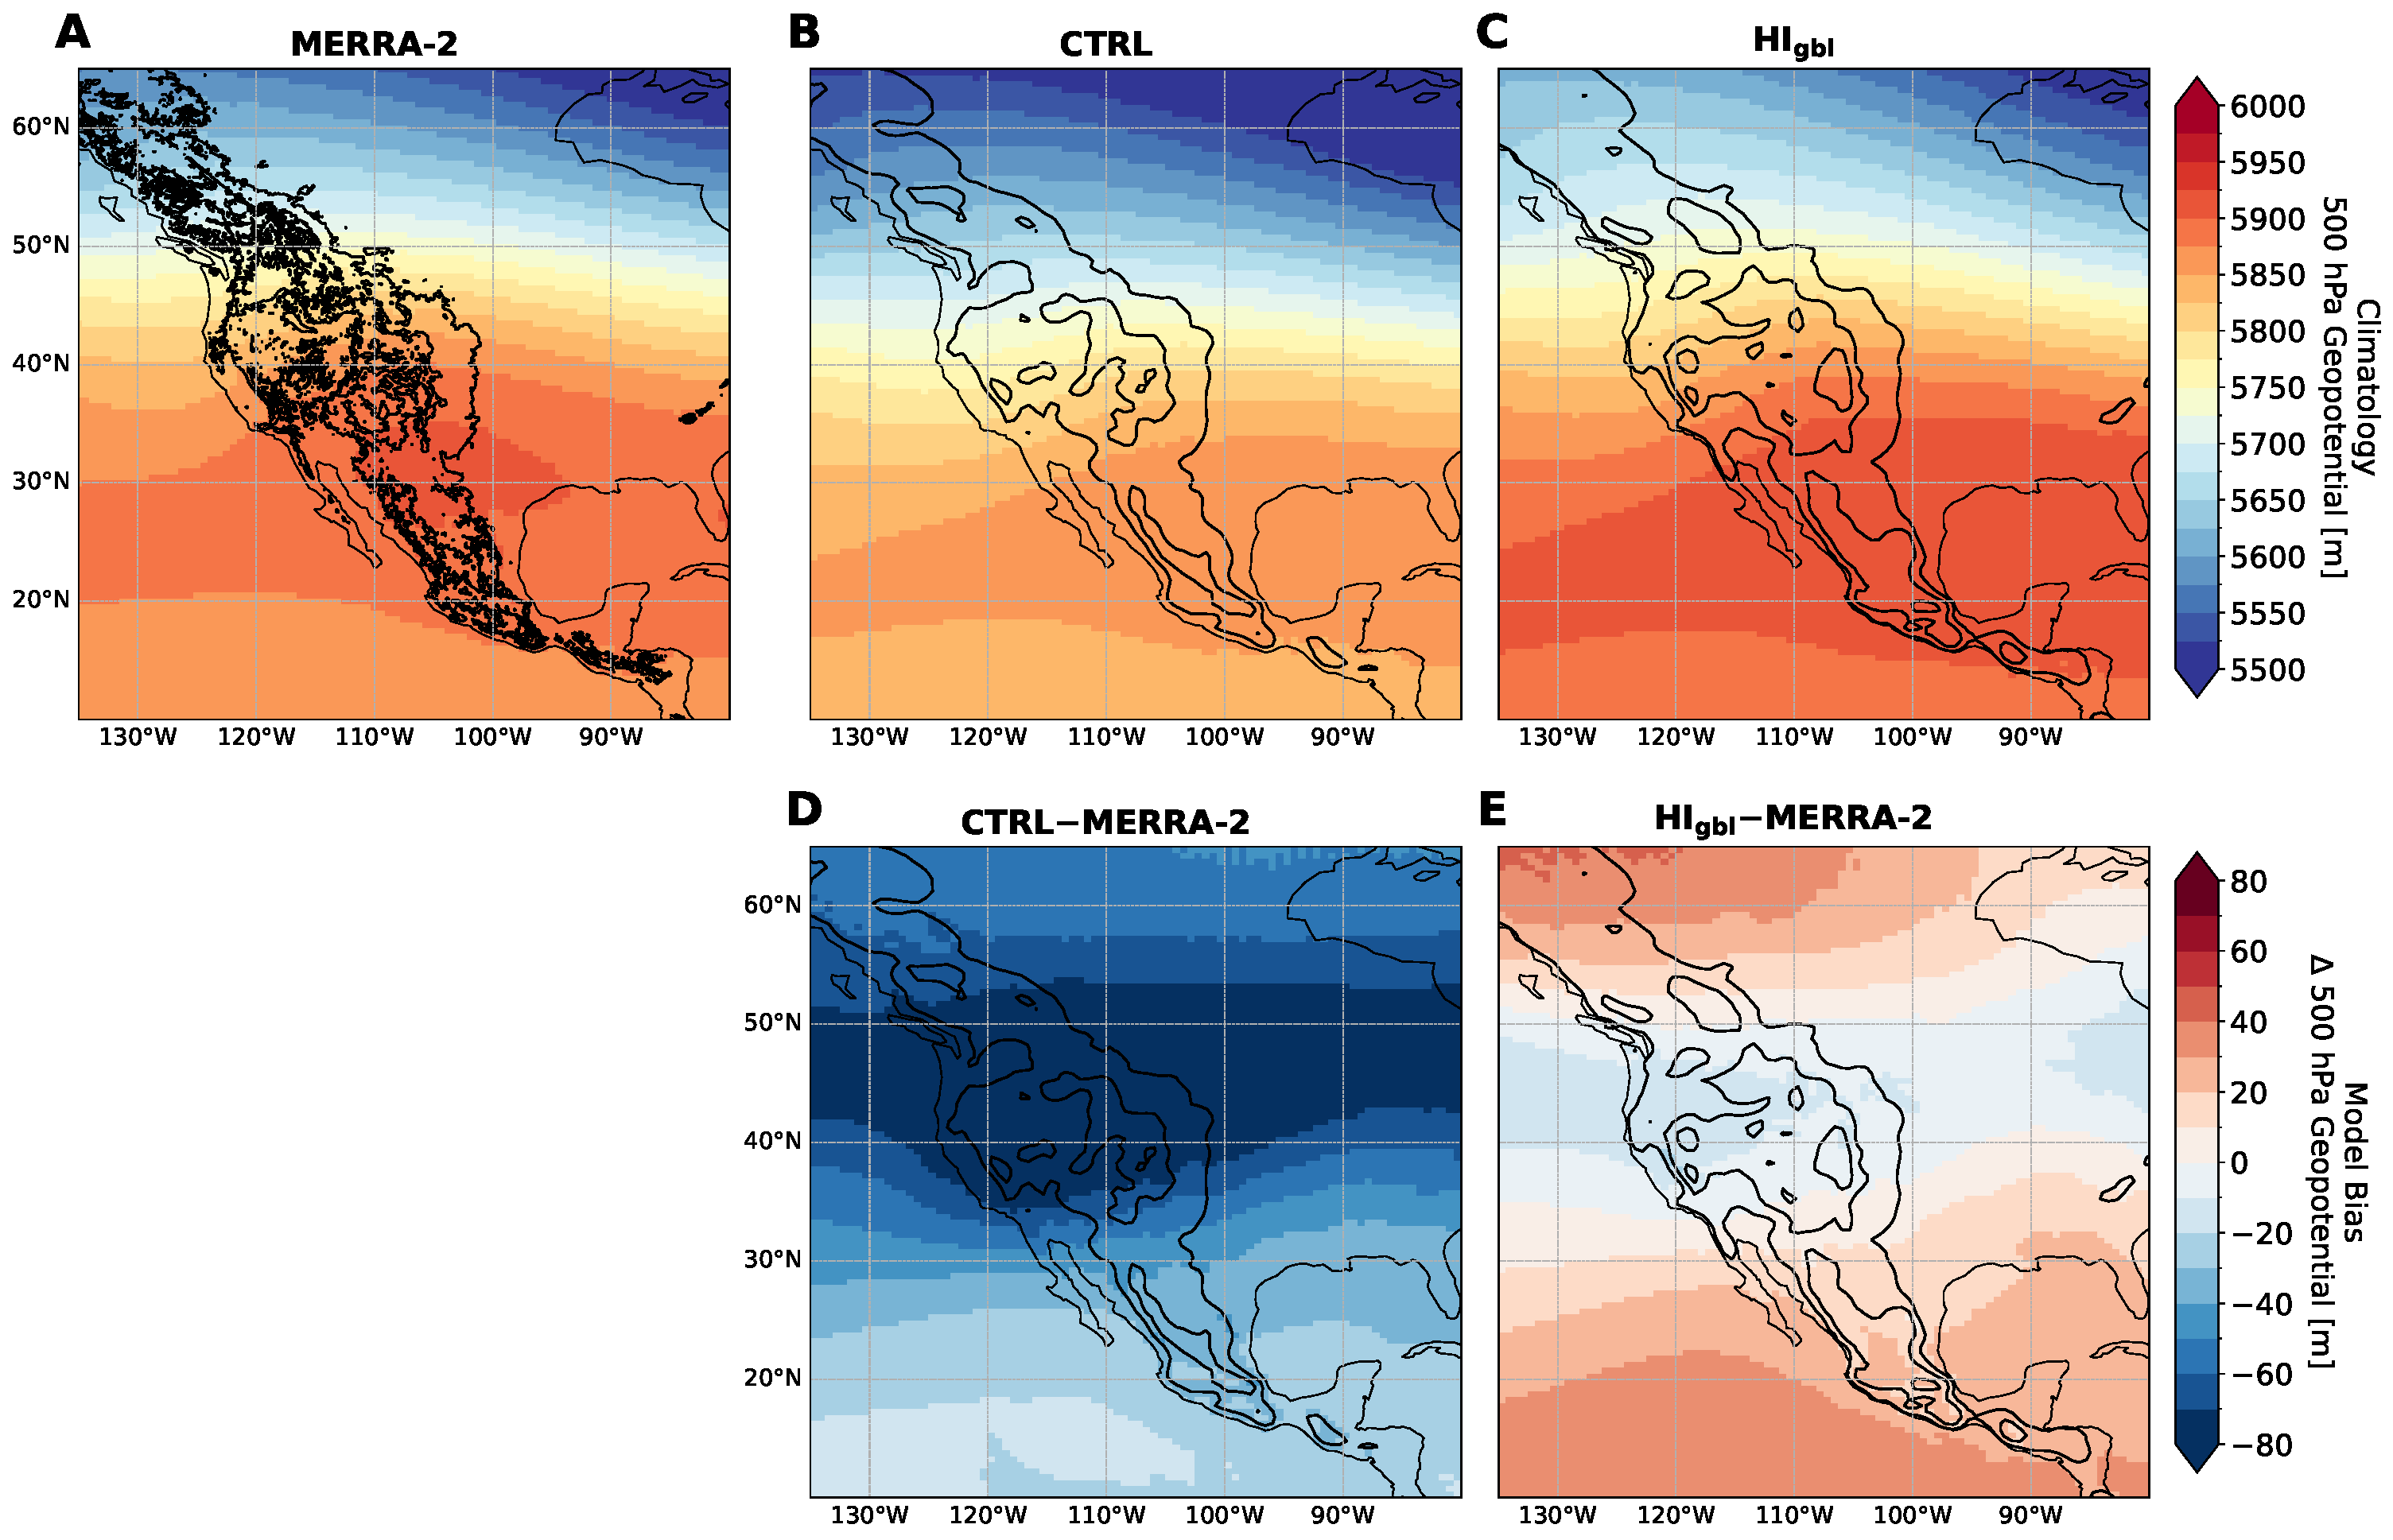
\includegraphics[width=\textwidth]{figs/fig_6_h500_swp_flor_pi_climo_merra2-bias.pdf}
    \caption{\textbf{Elevating North American topography in CM2.5-FLOR strengthens ridge in midtroposphere geopotential.} Climatological Jul.--Sept. mid-troposphere (500 hPa) geopotential heights ($\Phi_{500}$) in (a) MERRA-2 reanalysis, (b) CM2.5-FLOR CTRL, and (c) CM2.5-FLOR HI$_{gbl}$. The ridge of higher pressure over western North America in a--c corresponds to the ``Monsoon Ridge." Biases in CM2.5-FLOR's simulation of seasonal $\Phi_{500}$ relative to MERRA-2 when forced with (d) CTRL or (e) HI$_{gbl}$ topography. Thick black lines are topography contours between 1000 m and 4000 m, intervals of 1000 m.}
    \label{fig:flor-h500}
\end{figure}

One NAM-relevant topographic feature in HI$_{gbl}$ that was perturbed beyond what was in HI$_{mex}$ is the North American Cordillera, which is an important control on the large-scale circulation. As seasonal insolation forcing drives a larger fractional warming of the tropospheric column over elevated terrain \cite{higgins04jc,johnson25pdt}, the northwestward expansion of the monsoon ridge over the continent may thus be underestimated in CTRL due to too-low North American Cordillera peak heights. Indeed, we find that simulated 500 hPa geopotential heights better match reanalysis in HI$_{gbl}$ than CTRL (Figure \ref{fig:flor-h500}b,c), with reduced biases in its strength and position (Figure \ref{fig:flor-h500}d,e). The generation of an upper-level anticyclone due to the thermal effects of topography is also dynamically coupled to the strength of the lower-level cyclone \cite{hoskins91tdmo,rowson92ijc,rodwell01jc}. This expansion of the monsoon ridge may thereby explain the improved surface pressure patterns and thus stronger southerly flow in the GoCLLJ region. 

A more local feature, the Baja Peninsula, was also elevated in HI$_{gbl}$ but not HI$_{mex}$ as the western limit of the region with elevated terrain in HI$_{mex}$ was 113\textdegree{W}. Topography along the Baja Peninsula, particularly at its northern end, influences the development of the surface thermal low over the southwestern U.S. deserts by blocking the eastward movement of stable Pacific air masses and channelizing low-level winds to its east. We do not isolate the role of the Baja Peninsula directly in this study; additional perturbation experiments with topography elevated exclusively over the Baja Peninsula versus North America are necessary to definitively evaluate the relative roles of each feature in contributing to the enhanced along-Gulf SLP gradient. Though that is beyond the scope of this study, we hypothesize that topography in the Baja Peninsula may also play a substantive role in the increased sensitivity of the GoCLLJ to the SLP gradient in HI$_{gbl}$.


%% -------------------
\subsection{NAM Projections}
%% -------------------
Uncertainties in the baseline simulation of the NAM undermine confidence in model projections of future NAM rainfall \cite{pascale17ncc}. As shown above, better capturing the terrain-forced circulation of the NAM by increasing model spatial resolution or elevating resolved topography can lead to better simulation of NAM rainfall (though still with some biases in the spatial distribution of this rainfall). Next, we analyze whether HighResMIP and CM2.5-FLOR models' response to enhanced greenhouse gas forcing differently impacts NAM rainfall projections between models with better or worse simulation of historical NAM climatology. 

%% -------------------
\subsubsection{HighResMIP mid-century}

\begin{figure}[!htbp]
    \centering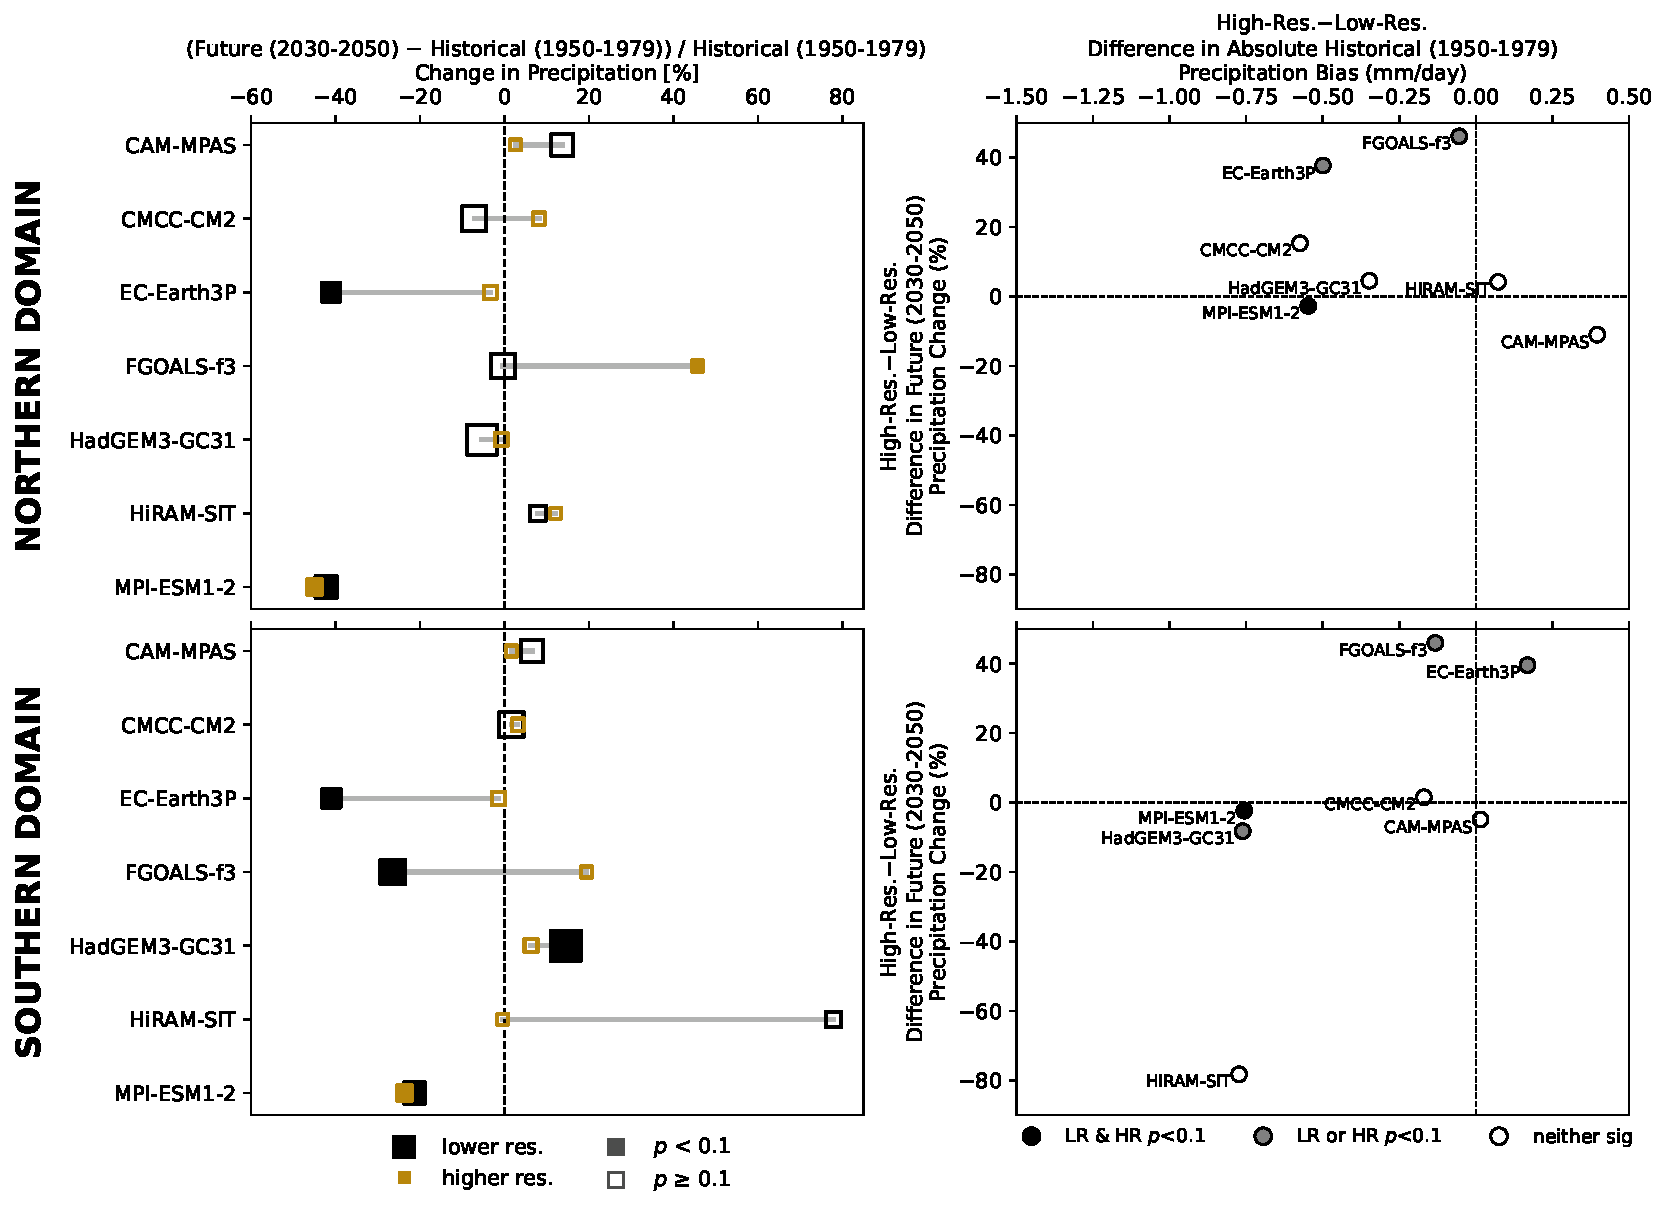
\includegraphics[width=\textwidth]{figs/fig_7_prec_hrmip_future_delta_1950-1979_vs_2030-2050.pdf}
    \caption{\textbf{Impact of resolution refinement on projected NAM rainfall in HighResMIP models.} HighResMIP models' projected change in mid-21st century relative to mid-20th century rainfall normalized against the mid-20th century rainfall climatology for the (a) Northern and (b) Southern Domains. Relationship between the impact of increased horizontal resolution on the absolute magnitude of models' historical precipitation biases and the magnitude of future relative precipitation change for the (c) Northern and (d) Southern Domains. Solid (open) markers indicate where the future change is statistically significant (insignificant) at the 10\% level (p$<$0.1) based on a two-sided Welch's t-test. In panels (c) and (d), circle colors further indicate whether the projected mid-century rainfall change is statistically significant (p$<$0.1) for both model configurations (black), either the low- or high-resolution configuration (grey), or neither configuration (white).}
    \label{fig:future-prec-hrmip}
\end{figure}

For the subset of HighResMIP models that contributed future simulations (CAM-MPAS, CMCC-CM2, EC-Earth3P, FGOALS-f3, HadGEM3-GC31, HiRAM-SIT, and MPI-ESM1-2), increasing spatial resolution predominantly led to higher rainfall rates in both the Northern and Southern Domains under historical greenhouse gas forcing (Figure \ref{fig:hrmip-biases}b,c). Yet, there is a lack of consensus among this subset of models in regard to the impacts of increased spatial resolution on their projections of NAM rainfall under enhanced greenhouse gas forcing and SST warming (Figure \ref{fig:future-prec-hrmip}). Resolution refinement leads to a greater relative increase or no change in future precipitation compared to the mid-20th century in both the Northern and Southern Domains in 3 models (CMCC-CM2, EC-Earth3P, FGOALS-f3) but to enhanced drying in both domains in 2 models (CAM-MPAS  and MPI-ESM1-2). The impact of resolution refinement on precipitation differs between domains for the remaining two models (HiRAM-SIT and HadGEM-GC31). 

Overall, we find that for models in which increasing resolution reduced domain-mean precipitation biases over the historical period (more negative values on x-axes of panels c and d on Figures \ref{fig:future-prec-hrmip}, S7, and S8), increasing resolution generally led to relative wetting in the Northern Domain but relative drying in the Southern Domain by the mid-21st century. This is suggestive that models with improved NAM simulation will have more wetting in the Northern Domain and drying in the Southern Domain. A challenge to interpreting these results is that the majority of projected changes in rainfall are statistically insignificant relative to interannual variability. Adjusting the averaging period used to define the historical and future climatologies results in qualitatively similar projected rainfall changes but reduces the number of models showing statistically significant differences, particularly in the Southern Domain (Figure S7 and S8). Due to the limitations of the length of the HighResMIP simulations, there is a fundamental trade-off between averaging across enough time so as to dampen noise from internal variability but maximizing the forcing effect between the future and historical periods. As such, the change in forcing between time periods is likely maximized to the extent possible for the climatologies as calculated in Figure \ref{fig:future-prec-hrmip}. 


%% -------------------
\subsubsection{CM2.5-FLOR 2$\times$CO$_2$}

\begin{figure}[!htbp]
    \centering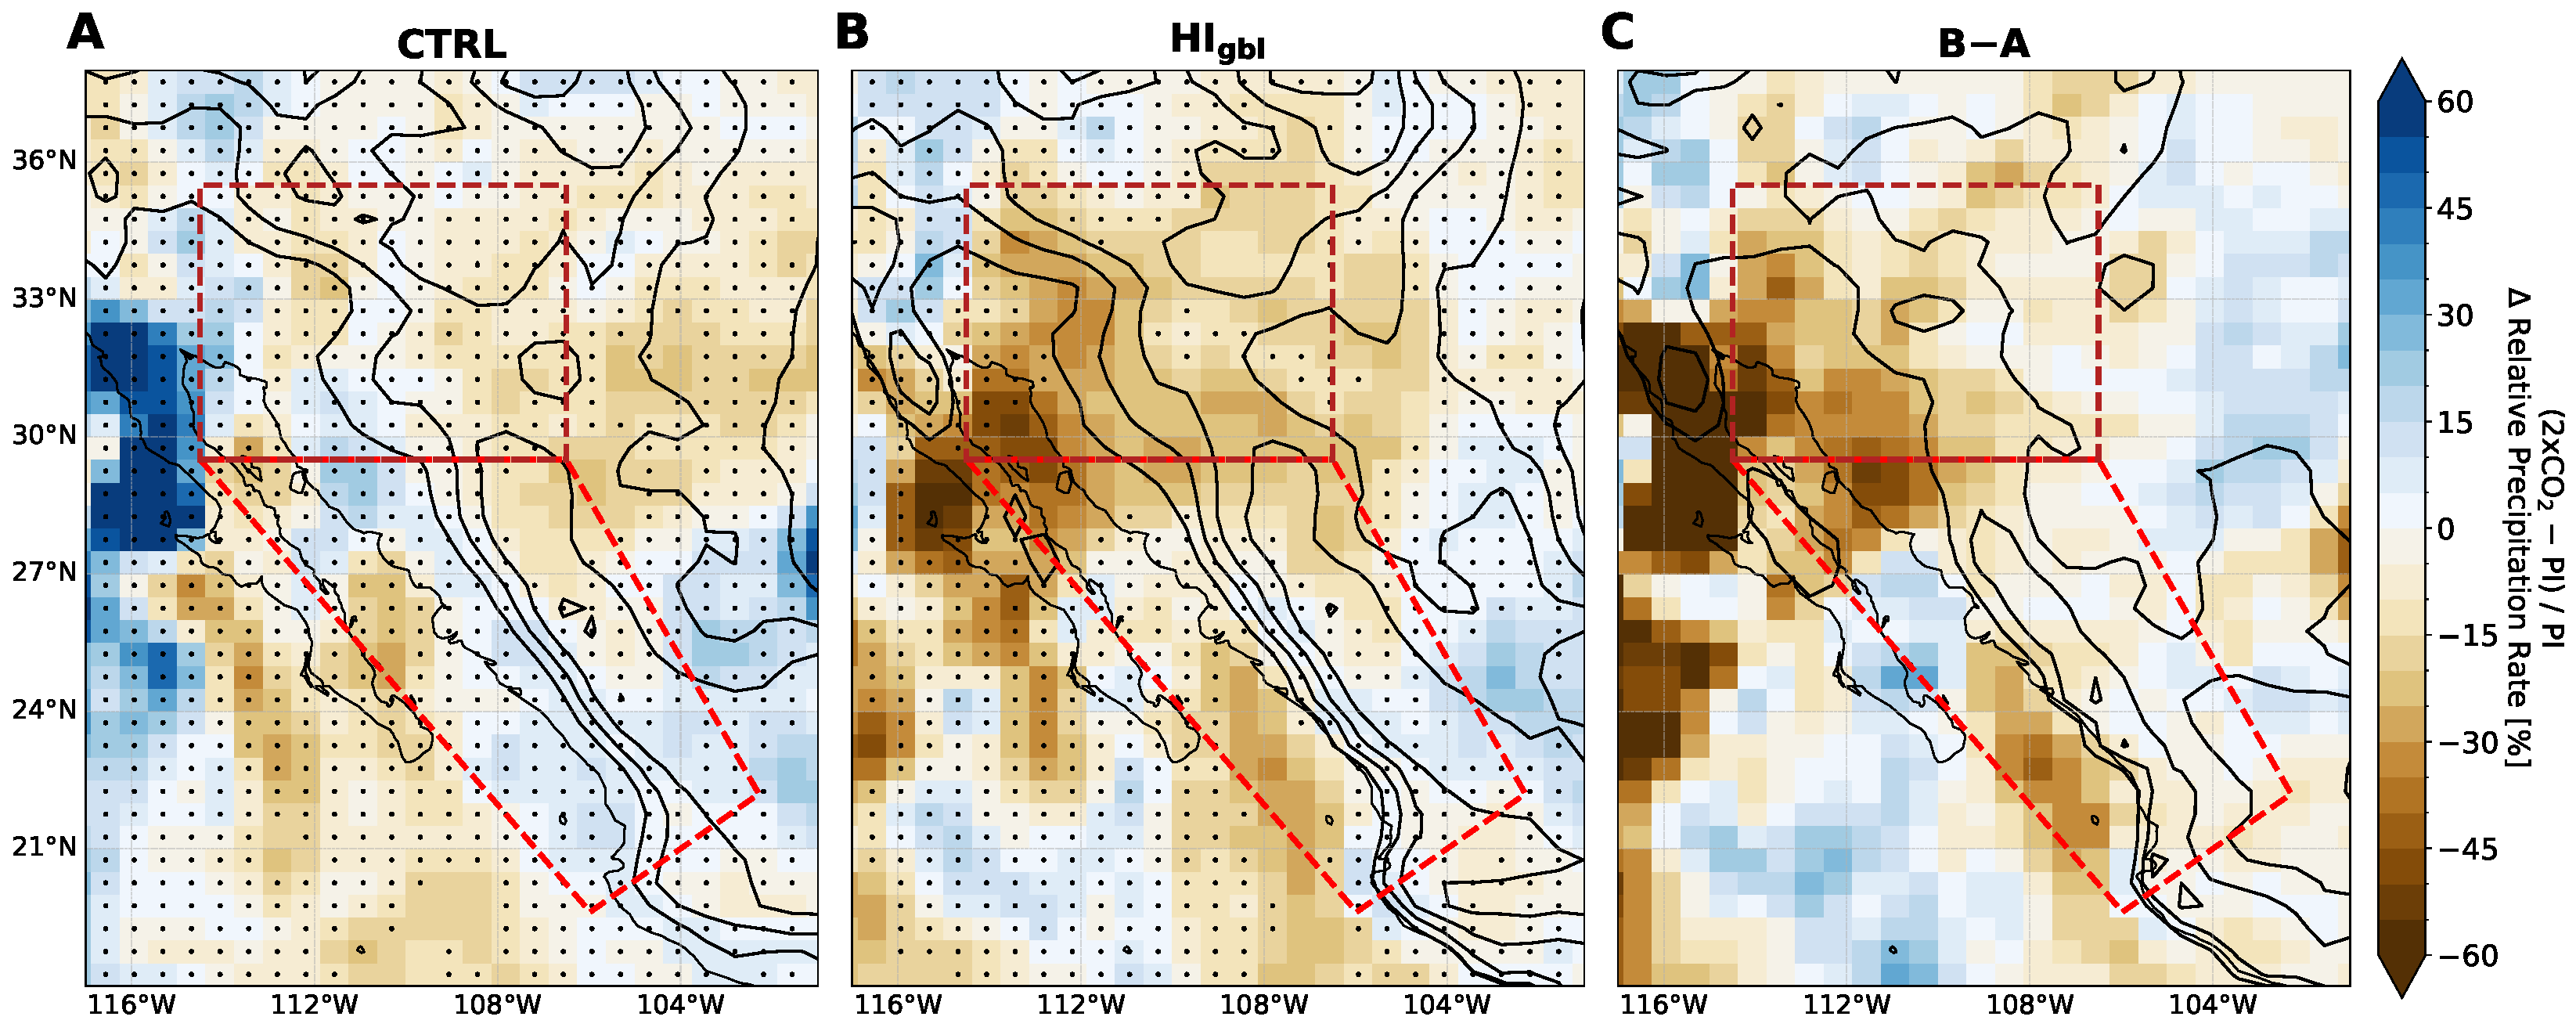
\includegraphics[width=\textwidth]{figs/fig_8_prec_flor_2xco2_pct_change.pdf}
    \caption{\textbf{Enhanced future drying in response to 2$\times$CO$_2$ forcing in CM2.5-FLOR with elevated topography.} Projected changes in Jul.--Sept. rainfall in response to 2$\times$CO$_2$ forcing relative to Preindustrial rainfall rates in CM2.5-FLOR forced with (a) CTRL or (b) HI$_{gbl}$ boundary conditions, and (c) the difference between projected changes in HI$_{gbl}$ and CTRL showing the impact of elevated topography on the response of NAM rainfall to elevated greenhouse gas forcing. Stippling on a--b covers regions where the relative change in rainfall is not statistically significant (p$>$0.1) based on a students's two-sided t-test. Dashed boxes outline the Northern (dark red) and Southern (light red) Domains. Thick black lines contour model topography from m to m, intervals of m.}
    \label{fig:flor-prec-future}
\end{figure}

Future climatologies for CM2.5-FLOR were calculated from 100 model years after CO$_{2}$ doubling was reached across which the radiative forcing was held constant at the 2$\times$CO$_2$ level. The stronger change in forcing between Preindustrial $p$CO$_2$ and 2$\times$CO$_2$, in addition to the greater length of time integrated, should minimize the impacts of internal variability on detection of the forced signal. CM2.5-FLOR with standard topographic boundary conditions (CTRL) nevertheless projects largely statistically insignificant changes in rainfall under 2$\times$CO$_2$ forcing outside of a small region of modest drying ($\sim$15\%) in the state of Chihuahua, Mexico (Figure \ref{fig:flor-prec-future}a). With a more accurate baseline NAM simulation (particularly at lower elevations) in HI$_{gbl}$, we find that the magnitude and extent of statistically significant future drying is enhanced reaching 30-50\% drying (Figure \ref{fig:flor-prec-future}b). The elevated topography in HI$_{gbl}$ has the greatest impact on future drying across a broad swath of southwest North America north of $\sim$27\textdegree{N}, encompassing northwestern Mexico, the northern Gulf of California, the Baja Peninsula, and southwestern Arizona (Figure \ref{fig:flor-prec-future}c). 


%% -------------------
\section{Discussion}
%% -------------------
In the subsequent sections, we further contextualize our results within the existing literature on the NAM, highlighting areas of consistency and divergence regarding model biases and projections of this phenomenon. Where our results agree with existing literature, they lend robustness to our understanding of the sources of model biases and the implications of refining horizontal resolution or topographic representation on them. Aspects for which there is divergence between our results and the current state of knowledge provide insights to sources of uncertainty on the dominant processes that influence NAM simulation.

%% -------------------
\subsection{Precipitation biases in the Southern Domain}
At low-resolutions, forced atmosphere models generally succeed in capturing the timing of peak NAM precipitation but inadequately capture its magnitude (Figure S2). With increasing resolution, there is better simulation of the mean rate of NAM precipitation in the Southern Domain, but the spatial distribution of that rainfall is at odds with observations; simulated rainfall is located too far upslope with insufficient amounts over the Gulf of California. Both the better resolution of topography and the Gulf of California may contribute to shifts in simulated precipitation following resolution enhancement of HighResMIP models. The exceptionally warm SSTs typical of the Gulf of California in boreal summer contribute to the high moist static energy of the overlying near-surface airmasses. Terrain-induced circulations---greater heating of elevated mountains during the day and mechanically-forced stationary wave patterns \cite{boos21n}---stimulate the eastward flow of these airmasses and their orographic lifting upon encountering the Sierra Madre Occidental, which ultimately allows for moist convection \cite{varuolo-clarke19jc,boos21n}. Though the high-resolution configurations somewhat succeed in simulating this process as they do produce precipitation in the western Sierra Madre in the Southern Domain (i.e., high MSE air was lifted in some capacity), they are biased in the sense that the exact location of the precipitation is incorrect (too far inland). We hypothesized that the spatial pattern of the lingering biases is due to incomplete representation of topographic blocking by the Sierra Madre Occidentals. 

We evaluated this hypothesis with the CM2.5-FLOR sensitivity experiments. Precipitation along the lower elevation slopes of the Sierra Madre Occidental is increased in both HI$_{gbl}$ and HI$_{mex}$. As such, we conclude that elevating Sierra Madre Occidental peak heights led to more rainfall along the lower Sierra Madre Occidental slopes in HI$_{gbl}$ by enhancing orographically-induced rainfall closer to the Gulf of California coast. This shift is consistent with the $\sim$50 km westward shift of Sierra Madre Occidental peak heights in HI$_{gbl}$ (and HI$_{mex}$) relative to CTRL, in better alignment with the observed location of topographic peak heights (Figure \ref{fig:topo}h). The changes in precipitation over the Sierra Madre Occidental in HI$_{gbl}$ and HI$_{mex}$ are thus consistent with the mechanism of elevated range heights enhancing orographically-induced convection along their lower windward slopes. 

Despite these improvements, the model still simulates excessive precipitation in the uppermost windward slopes in both sensitivity experiments (see hatching in Figure \ref{fig:flor-prec}b,c along the Sierra Madre Occidental's slopes $>$1 km masl north of $\sim$25\textdegree{N}) and too little over the low-lying plains and Gulf of California to the west. This could be due to the competing effects of elevating topography on flow blocking: elevating the height of the barrier would increase blocking of incident low-level winds all else being equal \cite{galewsky08jas}, however, it also enhances the mechanically forced stationary wave pattern that stimulates anomalous westerly flow \cite{ringler99jas,boos21n}. As such, the upslope direction of the anomalous westerlies might can partially compensate for the increased barrier heights and reduce its blocking efficacy.% The relative sensitivity of a model's circulation at 700 hPa may thus dictate how effective the increase in topographic forcing is in imparting flow blocking. 

Unrealistically strong westerly flow impinging on the windward flanks of the Sierra Madre Occidental due to an exaggerated stationary wave response may additionally counteract the nighttime downslope easterly flow that leads to the diurnal cycle of precipitation over the low-lying plains and Gulf of California \cite{berbery01jc,nesbitt08jh,castro12jc}. This effect may explain the exacerbation of model dry biases over the low-lying Gulf of California in HI$_{gbl}$ and HI$_{mex}$. \citeA{lee07jc} specifically evaluated the impact of increasing horizontal resolution from $\sim$2\textdegree{} to $\sim$0.5\textdegree{} in a small subset of atmosphere models on the diurnal cycle of the NAM and similarly found that resolution refinement led to relatively better simulation of upslope orographic processes than that of nighttime downslope flow over the Sierra Madre Occidental. The persistent underperformance in simulation of downslope flow over generations of model advancement suggests that more work is needed to adequately represent the processes that drive the downslope propagation of convection on diurnal timescales.

Transient eddies that compensate for time-mean moisture convergence and lower the balance of precipitation over the Sierra Madre Occidental \cite{boos21n} may also be underrepresented in CM2.5-FLOR, however, this explanation does not account for the exacerbated dry biases over the Gulf of California. The impact of altered topography on mechanically-forced stationary wave response ultimately provides a harmonious explanation of both the persistent excessive time-mean precipitation biases along the high-elevation Sierra Madre Occidental slopes and the underestimation of precipitation over the Gulf of California. This effect may be exaggerated in the CM2.5-FLOR sensitivity experiments due to the extreme nature of the grid-cell maximum topographic modification employed; prior work has shown that ``envelope'' based interpolation schemes provide a more moderate alteration to topographic boundary conditions that model developers may realistically consider \cite{meegan-kumar25jc}.

%% -------------------
\subsection{Precipitation biases in the Northern Domain}
Unlike the Southern Domain, resolution refinement has a lesser impact on simulated precipitation biases in the Northern Domain among HighResMIP models: both ensembles are too dry overall, and increasing resolution only reduces biases in 7 out of 15 model families. This result adds uncertainty to existing literature demonstrating increased horizontal resolution leads to an improvement of rainfall biases in the Northern Domain via enhanced low-level moisture convergence. Our finding that HighResMIP atmosphere models have recalcitrant dry biases in the Northern Domain even after resolution refinement and in the absence of SST biases suggests that these models are still lacking in their simulation of some process driving precipitation in the region that appears to be relatively insensitive to resolution variations within the range of HighResMIP. Persistent underestimation of regional topography even in the high-resolution configurations may result in the lack of necessary pieces to horizontally advect enthalpy that drives convection in the Northern Domain \cite{pascale18jc,varuolo-clarke19jc,johnson23jc}.

The CM2.5-FLOR sensitivity experiments, again, shed light on the influence of topography on the lingering biases in the high-resolution HighResMIP models. In these experiments, we believe three different topographic features---the Sierra Madre, Colorado Plateau, and Baja Peninsula---are most likely to be influencing the GoCLLJ, which predominantly drives moisture convergence in the Northern Domain. As we do not see a strengthening of the GoCLLJ in HI$_{mex}$, elevating the Sierra Madre Occidental alone is insufficient to impact its simulation. Our results support prior work identifying the relevance of topography in the Baja Peninsula and/or larger North American continent on moisture convergence north of the Gulf of California \cite{tang84mwr,anderson00bjgra,newman12mwr,pascale16jc,varuolo-clarke19jc,johnson23jc,johnson25pdt}. While we examine monthly data in this study, in reality bursts in precipitation frequency and intensity in the Northern Domain have been shown to result from surges of the GoCLLJ connected to midlatitude systems propagating eastward across North America on synoptic timescales \cite{stensrud97mwr,pascale16mwr,pascale16jc}. Improvements to the simulation of the mean and monthly variation of southerly winds and moisture convergence in the Northern Domain in HI$_{gbl}$ are therefore likely related to sufficient improvements in simulation of the GoCLLJ and its synoptic drivers \cite{mullen98mwr,turrent09grl,castro12jc,pascale16jc,pascale18jc}. We do indeed find a northwestward shift of the monsoon ridge HI$_{gbl}$ such that its mean intensity and position are more aligned with observations (Figure \ref{fig:flor-h500}e). 

There is a potential additional role for the Baja Peninsula acting as a barrier in the west that helps to channelize the southerly flow arising from the along-Gulf SLP gradient \cite{pascale16jc}. The importance of northern Baja topography may explain why the GoCLLJ is more sensitive to variations in the along-Gulf SLP gradient in HI$_{gbl}$ compared to HI$_{mex}$ (Figure \ref{fig:flor-slp-llj}f). As orographic blocking by Baja Peninsula topography and the strengthening of the mid-tropospheric ridge by elevating North American topography have similar impacts on surface low deepening in the northern NAM domain, we cannot disentangle the relative contributions of these two mechanisms to the change in circulation in HI$_{gbl}$. Nevertheless, the elevation of topography in both regions is consistent with the enhanced GoCLLJ strength and moisture convergence in the northern NAM domain.

Land surface memory can additionally modulate summertime circulation in southwestern North America. North American topography shapes wintertime circulation patterns through the deflection of the westerly storm tracks. This creates a strong rain shadow between the coastal and interior U.S. \cite{johnson25jc,sexton26jc} that, in turn, leads to low spring soil moisture conditions antecedent to NAM onset. Soil moisture ultimately mediates land-atmosphere coupled processes that influence the strength and position of the surface thermal low and monsoon ridge and their feedbacks \cite{higgins00jc,grantz07jc,zhu07jc,notaro11grl,cerezo-mota16ijc,zeppetello24jc}. The latest generations of CMIP5 and CMIP6 GCMs show excessive wintertime precipitation \cite{sexton26jc} and springtime soil moisture \cite{hernandez22jgra} in southwestern North America, consistent with a reduced rain shadow. Enhanced blocking of westerly storms during wintertime by the elevated North American terrain in HI$_{gbl}$ may have additionally pre-conditioned the land surface to warming at the onset of summer \cite{cerezo-mota16ijc} and thus set up the self-reinforcing circulation even after onset of NAM rainfall.  %To verify this, Ben Johnson suggests: To see if the winter precip is having a land feedback effect in the winter, I'd plot both the evaporation and precipitation change. If evaporation increases more than precipitation in the summer, then this suggests that the prior higher soil moisture has an impact during the summer.

%% -------------------
\subsection{Role of horizontal resolution and orographic blocking on future NAM projections}
CMIP5 and CMIP6 multi-model ensemble projections showing reduced precipitation during the peak NAM season (Jul.--Sept.) point to an overall drier NAM in the future \cite{cook13jgra,pascale17ncc,hernandez22jgra,ye23jc}. But, variety across projections in the direction of future NAM rainfall reflects a balance between the relative impacts of land-surface drying versus enhanced moisture convergence from oceanic sources in the future (xx,xx). Faith in these projections is undermined by general NAM simulations biases discussed in prior sections.

Statistically and dynamically downscaled regional climate models, however, suggest that increased evaporation from the Gulf of California can overcome the impact of elevated surface temperatures on land surface drying such that the NAM will intensify in response to increased greenhouse gases \cite{meyer17cd,wallace24cd,nazarian24jc,kim24ijc}. SST biases that influence land-sea thermal contrast, atmospheric stability, and thus large-scale circulation patterns are also influential on NAM projections \cite{higgins00jc,turrent09grl,bukovsky15jc,ye23jc}. Biases in simulated large-scale circulation patterns in GCMs are additionally known to be inherited during downscaling of regional circulation models that undermines their skill in capturing the NAM \cite{castro12jc,cerezo-mota16ijc}. Disagreement among models regarding which process will dominate the regional response to rising greenhouse gases precludes confidence in our understanding of future changes in the NAM.

Those that better simulate the present day NAM might be considered to have more credible projections \cite{bukovsky15jc}. Here, we explored two different types of projections that provide distinct insights into the impact of bias reduction in the simulation of the historical NAM alters future projections: the HighResMIP ensemble forced with SSP5-8.5 greenhouse gas emissions and the CM2.5-FLOR simulations forced with 2$\times CO_{2}$. The HighResMIP ensemble explores the influence of resolution refinement while the CM2.5-FLOR simulations demonstrate the effects of resolving certain lingering model biases associated with topography that remain at high-resolutions on rainfall projections.

The sign of future rainfall change as well as the impact of increasing horizontal resolution on that change in HighResMIP is largely statistically insignificant ($p\geq0.1$) relative to interannual variability during the historical period. Though the conclusions inferred from the HighResMIP models are thus equivocal, the subset of models in which resolution refinement led to a reduction in domain-mean biases in historical precipitation simulation generally agree on less drying/more wetting in the Northern Domain and more drying in the Southern Domain by the mid-21st century compared to the mid-20th century. 

This impact of increased resolution on the response to increased greenhouse gas forcing is distinct from that following topographic perturbation in CM2.5-FLOR. When the implementation of grid-cell maximum topography in HI$_{gbl}$ alleviates lingering Preindustrial mean state biases, we observe more future drying in the Northern and Southern Domains in response to 2$\times$CO$_2$, though the magnitude of future drying is greater in the Northern Domain. So while both modifications can yield improved simulations of the modern NAM, increasing horizontal resolution and explicitly maximizing orographic processes appear to have differing impacts on the response of the NAM to elevated greenhouse gas forcing, particularly in the Northern Domain. 

Though these results are distinct from one another, they are not at odds with prior work on impact of reduced model biases on these projections. Prior work specifically looking across the CM2.5 family of models at increasing resolution similarly found 2$\times$CO$_2$ forcing led to progressively higher rainfall rates in the Arizona-New Mexico region (our Northern Domain) during Jun.--Aug. \cite{van-der-wiel16jc}. These results conform with the HighResMIP ensemble, suggesting that increased resolution generally leads to relatively wetter future conditions in the Northern Domain. \citeA{pascale17ncc,pascale18jc} found that reducing SST biases in the CM2.5-FLOR model through flux-adjustments enhances future NAM drying due to lowered specific humidity over land by amplified warming that suppressed precipitation. \citeA{baldwin21a} has previously demonstrated that HI$_{gbl}$ topography also reduces mean state SST biases in CM2.5-FLOR, which suggests that the results of this experiment are consistent with those from Pascale et al. 

Importantly, \citeA{pascale17ncc} found that CM2.5-FLOR specifically simulated weak future drying in the NAM region under 2$\times$CO$_2$ forcing due to model SST biases that drove late-season increases in evaporation, and consequently, moist static energy that compensated for higher surface radiation fluxes. Flux-adjusting SST in CM2.5-FLOR decreased atmospheric buoyancy, which suppresses convection, over the Sierra Madre Occidental and southwest U.S. under the same forcing. The ability of the land surface to sustain convection via the impact of evapotranspiration on atmospheric instability was therefore reduced under higher CO$_{2}$ forcing in the flux-adjusted CM2.5-FLOR model, leading to more persistent future drying. As such, although increasing horizontal resolution in the flux-adjusted CM2.5 model similarly increased moisture convergence in the Northern Domain, lowered specific humidity due to amplified warming over land ultimately suppressed precipitation. Near-surface saturation specific humidity can thus also influence summer precipitation sensitivity to CO$_{2}$ forcing with increasing horizontal resolution \cite{pascale17ncc,pascale18jc} and the possible underestimation of the effects of warming on land surface and low-level drying in the HighResMIP ensemble and non-flux-adjusted CM2.5-FLOR model may result in precipitation overestimates. As the modified topography CM2.5-FLOR experiments described in this study did not incorporate flux adjustments, they may additionally underestimate the magnitude of future drying in response to 2$\times$CO$_2$.

This mechanism may additionally shed light on the effect of elevated topography on NAM rainfall projections in our elevated topography CM2.5-FLOR experiments. Despite elevated topography enhancing summertime precipitation, which would increase soil moisture, this increase might be less effective at sustaining high soil moisture conditions between episodic summer precipitation events when the antecedent soil moisture conditions are dry. As elevated topography reduces wintertime precipitation and springtime soil moisture due to deflection of the westerly storm tracks impinging on North America \cite{sextion26jc} in the Preindustrial and wintertime precipitation is robustly understood to decline with increased greenhouse gas forcing, the combined effects of these two processes on antecedent land surface conditions may considerably increase atmospheric stability over the continent in summertime in the future. 

As such, even though the inter-model spread across the HighResMIP ensemble creates uncertainty around the direction and magnitude of future NAM rainfall changes, the weight of evidence provided by our 2$\times$CO$_2$ experiments forced with HI$_{gbl}$ topography in addition to the flux-adjusted CM2.5 simulations from \citeA{pascale17ncc,pascale18jc} alongside expected increases in summertime temperatures that will exacerbate aridity, seem to point to a drier future climate in the NAM region.

%% -------------------
\section{Conclusions}
In this study, we deepen our understanding of the source of NAM biases in GCMs and the possible role of horizontal resolution and topography on those biases. First, we explored the relationship between global increases in horizontal resolution---and therefore the improved representation of topography in model boundary conditions---on NAM precipitation using paired simulations of SST-forced atmosphere models run at low- and high-resolutions from HighResMIP. Our analysis of HighResMIP models nuances the notion that increasing horizontal resolution improves model simulation of NAM precipitation in regions of complex terrain. Across model families, increased resolution does not consistently reduce dry biases in the Northern Domain and it restructures biases in the Southern Domain to exhibit a prominent dipole of negative and positive biases across the Sierra Madre topography. Given the persistent, though changed, nature of NAM precipitation biases in the high-resolution model configurations, we additionally explored sensitivity of one model (CM2.5-FLOR) to specific local orographic blocking by the Sierra Madre Occidental in northwest Mexico versus (thermo)dynamic processes associated with surrounding topography in western North America (the Baja Peninsula and North American Cordillera) using a set of idealized experiments forced with modified topographic boundary conditions that maximize topographic peak heights \cite<c.f.,>{baldwin21a,sexton26jc}. The CM2.5-FLOR sensitivity experiments (e.g., HI$_{gbl}$ vs. HI$_{mex}$) suggested that the lingering biases in the HighResMIP simulations stem from limited resolution of topographic peak heights and orographic blocking, even when models reach relatively high resolution ($\sim$50 km). These experiments additionally inform our understanding of which topographic features are most relevant as different elements of topography and their improved representation at higher resolutions have been invoked to be important in NAM simulation in past studies. 

We find direct orographic blocking by the Sierra Madre Occidental key for shaping the spatial pattern of precipitation in the Southern Domain. The impact of Baja and North American topography on continental-scale pressure fields additionally contributes to the simulation of realistic low-level circulation and precipitation patterns in the Northern Domain. This suggests that classic orographic upslope processes drive Southern Domain precipitation, but thermodynamic impacts of topography in Baja Peninsula and North America are necessary for capturing large-scale/continental-scale pressure patterns. Our results thus ultimately highlight the ``multi-scale nature of the NAM'' \cite{ye23jc}. To be clear, we are not asserting that the topographic modification implemented in HI$_{gbl}$ is a universal solution for improving simulations of summertime climate in North America as there are places where the elevated terrain worsens model biases, such as the front range of the Rocky Mountains. Rather, we emphasize that these sensitivity experiments suggest that a significant proportion of the precipitation biases remaining after resolution refinement of HighResMIP models are attributable to insufficient orographic blocking. 

In light of this deeper understanding, we evaluated how improvements in the simulation of the modern NAM due to resolution refinement and more realistic representations of orographic processes impact future projections of summer rainfall in southwest North America in both HighResMIP and the idealized CM2.5-FLOR experiments. Despite models with more realistic topographic forcing---due to either directly elevated topography or increased spatial resolution---showing similar improvements to the baseline simulation of NAM rainfall under present-day boundary conditions, the sign and magnitude of their future projections are inconsistent, with some suggesting intensification and others weakening. This lack of agreement may be due, in part, to the still strong imprint of internal variability on NAM rainfall. This underscores the need for long simulations and/or large ensembles in generating statistically robust projections of future NAM rainfall. Ultimately, the impact of land-atmosphere processes relative to thermodynamic increases in atmospheric moisture content will determine whether rainfall will increase or decrease in the future. The balance between these processes appears to vary substantially across model structures, complicating interpretations of NAM projections.


%%%%%%%%%%%%%%%%%%%%%%%%%%%%%%%%%%%%%%%%%%%%%%%
%% Optional Appendices go here
%
% The \appendix command resets counters and redefines section heads
%
% After typing \appendix
%
%\section{Here Is Appendix Title}
% will show
% A: Here Is Appendix Title
%
%\appendix
%\section{Here is a sample appendix}


%%%%%%%%%%%%%%%%%%%%%%%%%%%%%%%%%%%%%%%%%%%%%%%
% Acronyms
%% NOTE that acronyms in the final published version will be spelled out when used in figure captions.
%   \begin{acronyms}
%   \acro{Acronym}
%   Definition here
%   \acro{EMOS}
%   Ensemble model output statistics
%   \acro{ECMWF}
%   Centre for Medium-Range Weather Forecasts
%   \end{acronyms}


%%%%%%%%%%%%%%%%%%%%%%%%%%%%%%%%%%%%%%%%%%%%%%%
% DATA SECTION and ACKNOWLEDGMENTS
%%%%%%%%%%%%%%%%%%%%%%%%%%%%%%%%%%%%%%%%%%%%%%%

\section*{Open Research Section}
The HighResMIP data used in this study is freely available from the Earth System Grid Federation; the DOIs of the HighResMIP model output used in analyses are:
\begin{itemize}
    \item CAM-MPAS-LR \url{https://doi.org/}
    \item CAM-MPAS-HR \url{https://doi.org/}
    \item CAMS-CSM1-0-LR \url{https://doi.org/10.22033/ESGF/CMIP6.1399} %%%
    \item CAMS-CSM1-0 \url{https://doi.org/10.22033/ESGF/CMIP6.11003}
    \item CMCC-CM2-HR4 \url{https://doi.org/10.22033/ESGF/CMIP6.1359}
    \item CMCC-CM2-VHR4 \url{https://doi.org/10.22033/ESGF/CMIP6.1367}
    \item CNRM-CM6-1 \url{https://doi.org/10.22033/ESGF/CMIP6.1925} 
    \item CNRM-CM6-1-HR \url{https://doi.org/10.22033/ESGF/CMIP6.1387}
    \item EC-Earth-3P \url{https://doi.org/10.22033/ESGF/CMIP6.2322}
    \item EC-Earth-3P-HR \url{https://doi.org/10.22033/ESGF/CMIP6.2323}
    \item ECMWF-IFS-LR \url{https://doi.org/10.22033/ESGF/CMIP6.2463}
    \item ECMWF-IFS-HR \url{https://doi.org/10.22033/ESGF/CMIP6.2461}
    \item FGOALS-f3-L \url{https://doi.org/10.22033/ESGF/CMIP6.12001}
    \item FGOALS-f3-H \url{https://doi.org/10.22033/ESGF/CMIP6.2041}
    \item GFDL-CM4 \url{https://doi.org/10.22033/ESGF/CMIP6.1402} %%%
    \item GFDL-CM4C192 \url{https://doi.org/10.22033/ESGF/CMIP6.2262}
    \item HadGEM3-GC31-LM \url{https://doi.org/10.22033/ESGF/CMIP6.1321}
    \item HadGEM3-GC31-MM \url{https://doi.org/10.22033/ESGF/CMIP6.1902}
    \item HadGEM3-GC31-HM \url{https://doi.org/10.22033/ESGF/CMIP6.446}
    \item HiRAM-SIT-LR \url{https://doi.org/10.22033/ESGF/CMIP6.13303}
    \item HiRAM-SIT-HR \url{https://doi.org/10.22033/ESGF/CMIP6.13301}
    \item INM-CM5-0 \url{https://doi.org/10.22033/ESGF/CMIP6.1423} %%%
    \item INM-CM5-H \url{https://doi.org/10.22033/ESGF/CMIP6.14041}
    \item IPSL-CM6A-LR \url{https://doi.org/10.22033/ESGF/CMIP6.1534} %%%
    \item IPSL-CM6A-ATM-HR \url{https://doi.org/10.22033/ESGF/CMIP6.16361}
    \item MPI-ESM1-2-LR \url{https://doi.org/10.22033/ESGF/CMIP6.742} %%%
    \item MPI-ESM1-2-HR \url{https://doi.org/10.22033/ESGF/CMIP6.762}
    \item MPI-ESM1-2-XR \url{https://doi.org/10.22033/ESGF/CMIP6.10290}
    \item MRI-ESM2-0 \url{https://doi.org/10.22033/ESGF/CMIP6.621} %%%
    \item MRI-AGCM3-2-H \url{https://doi.org/10.22033/ESGF/CMIP6.10942}
    \item MRI-AGCM3-2-S \url{https://doi.org/10.22033/ESGF/CMIP6.1625}
    \item NICAM16-7S \url{https://doi.org/10.22033/ESGF/CMIP6.1033}
    \item NICAM16-8S \url{https://doi.org/10.22033/ESGF/CMIP6.1034}
\end{itemize}

Model output from the CM2.5-FLOR simulations CTRL, HI$_{mex}$ and HI$_{gbl}$ originally published in \citeA{baldwin21a} (experiments referred to as ``ctrl,'' ``hicam,'' and ``hitopo,'' respectively, in the original study) are available from the associated Zenodo repository at \url{https://doi.org/10.5281/zenodo.4619128}. Model output from the CM2.5-FLOR simulations presented for the first time as part of this study, as well as the observation and reanalysis data (IMERG, TRMM, GPCC, GPCP, MERRA-2) used for model evaluation and ETOPO05 topographic data, are provided in the Zenodo repository \url{https://doi.org/xxxxxxxxx}. Model code for CM2.5-FLOR is available from GFDL.... Code used for data analysis and figure creation is published on D.M.K.'s github \url{https://github.com/dervlamk/nam-topo-sensitivity}. 

\section*{Conflict of Interest}
The authors declare there are no conflicts of interest for this manuscript.

\acknowledgments
This work is supported by NASA NIP Grant 80NSSC21K1735 awarded to J.W.B. Computing resources for data analysis were provided by the NASA High-End Computing (HEC) Program through the NASA Center for Climate Simulation (NCCS) at the Goddard Space Flight Center.  We thank Gabriel Vecchi for supporting the running of the CM2.5-FLOR elevated topography simulations on Princeton's supercomputing system. We also thank Jared Sexton at the University of California Irvine for his help with the initial HighResMIP analyses in addition to Ben Johnson at Colorado State University for his insightful comments and aid in interpreting these results.

%%%%%%%%%%%%%%%%%%%%%%%%%%%%%%%%%%%%%%%%%%%%%%%
% REFERENCES and BIBLIOGRAPHY
%%%%%%%%%%%%%%%%%%%%%%%%%%%%%%%%%%%%%%%%%%%%%%%
\bibliography{high-res_hitopo_nam}

\end{document}